%! Author = melek
%! Date = 22.01.2023

% Preamble
\documentclass[11pt]{article}

% Packages
\usepackage{amsmath}
\usepackage{graphicx}
\graphicspath{ {../images/} }

\title{Assignment 5: Exploration Strategies and Offline Reinforcement Learning}
\author{huseyinabanox@gmail.com}
\date{February 2023}

% Document
\begin{document}

    \maketitle

    \section*{Observations}

    \subsection*{Truncated Episodes}

    Episodes have a maximum number of steps limit.
    An episode termination may be due to reaching the target or maximum number of limits.
    Provided implementation offers no detail about termination reason.

    If an episode terminates due to maximum step limit, it is said to be truncated.
    A truncated episode should use bootstrapped next state value in the target calculations.
    Upon reaching target, the desired termination, target calculations should not boostrap.

    Why this is important?
    We are already working in the so-called deadly-triad territory.
    Target calculations should be accurate to not increase the chance of divergence.

    As a solution, the environment is wrapped with a TimeLimit wrapper and truncated episodes are handled accordingly.

    \subsection*{Offline Training Returns}

    At each step, the agent selects an action, using the last observation, from the replay buffer, and steps the environment.

    Once offline training is switched on, data collection is turned off.
    The last observation in the replay buffer is not updated.
    The last observation and the actual environment state relation is broken.
    All the actions taken from that point on are literally blindly taken and observed training performance is a random product.

    It may be easy to fix the problem but may not worth it.
    Evaluation performance is sufficient and more important.
    Thus disregarding the training performance in the offline setting seems to be the most suitable action.

    \section*{Remarks}

    Each experiment is run using 4 different seeds and their average is displayed.
    Training return is average of the last 100 training step rewards.
    Evaluation return is average of the 1000 evaluation step rewards.

    \section*{Part 1: “Unsupervised” RND and exploration performance}

    \subsection*{RND Implementation}

    Experiments are run using easy, medium and hard environments.
    Relevant notebooks with plots can be found and report package.

    \subsubsection*{Easy Environment}

    Expectation 1: For debugging this problem, note that on the easy environment we would expect to obtain a mean reward (100 episodes) of -25 within 4000 iterations of online exploitation.

    Online exploitation starts after 10K iterations.
    Plus 4K iteration sums to 14K iteration.
    We are required to reach a mean reward of -25 within 14K iterations.

    \hspace*{-0.6in}
    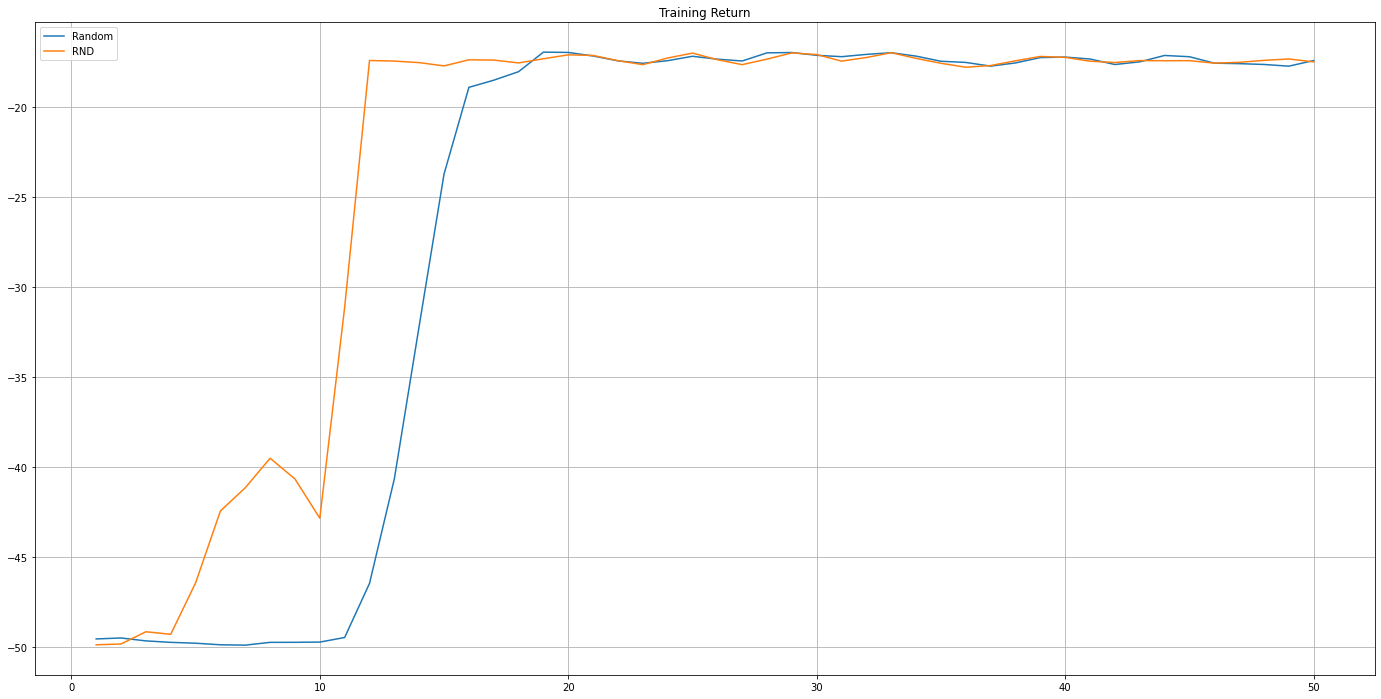
\includegraphics[scale=0.30]{q1/q1-easy-train-compare}

    The chart shows both exploration strategies reach the target mean reward within 14K iterations.
    The RND strategy reaches the target immediately after the beginning of the online exploitation.

    Expectation 2: The density of the state-action pairs on this easy environment is, as expected, more uniformly spread over the reachable parts of the environment (that are not occupied by walls) with RND as compared to random exploration where most of the density would be concentrated around the starting state.

    \hspace*{-0.6in}
    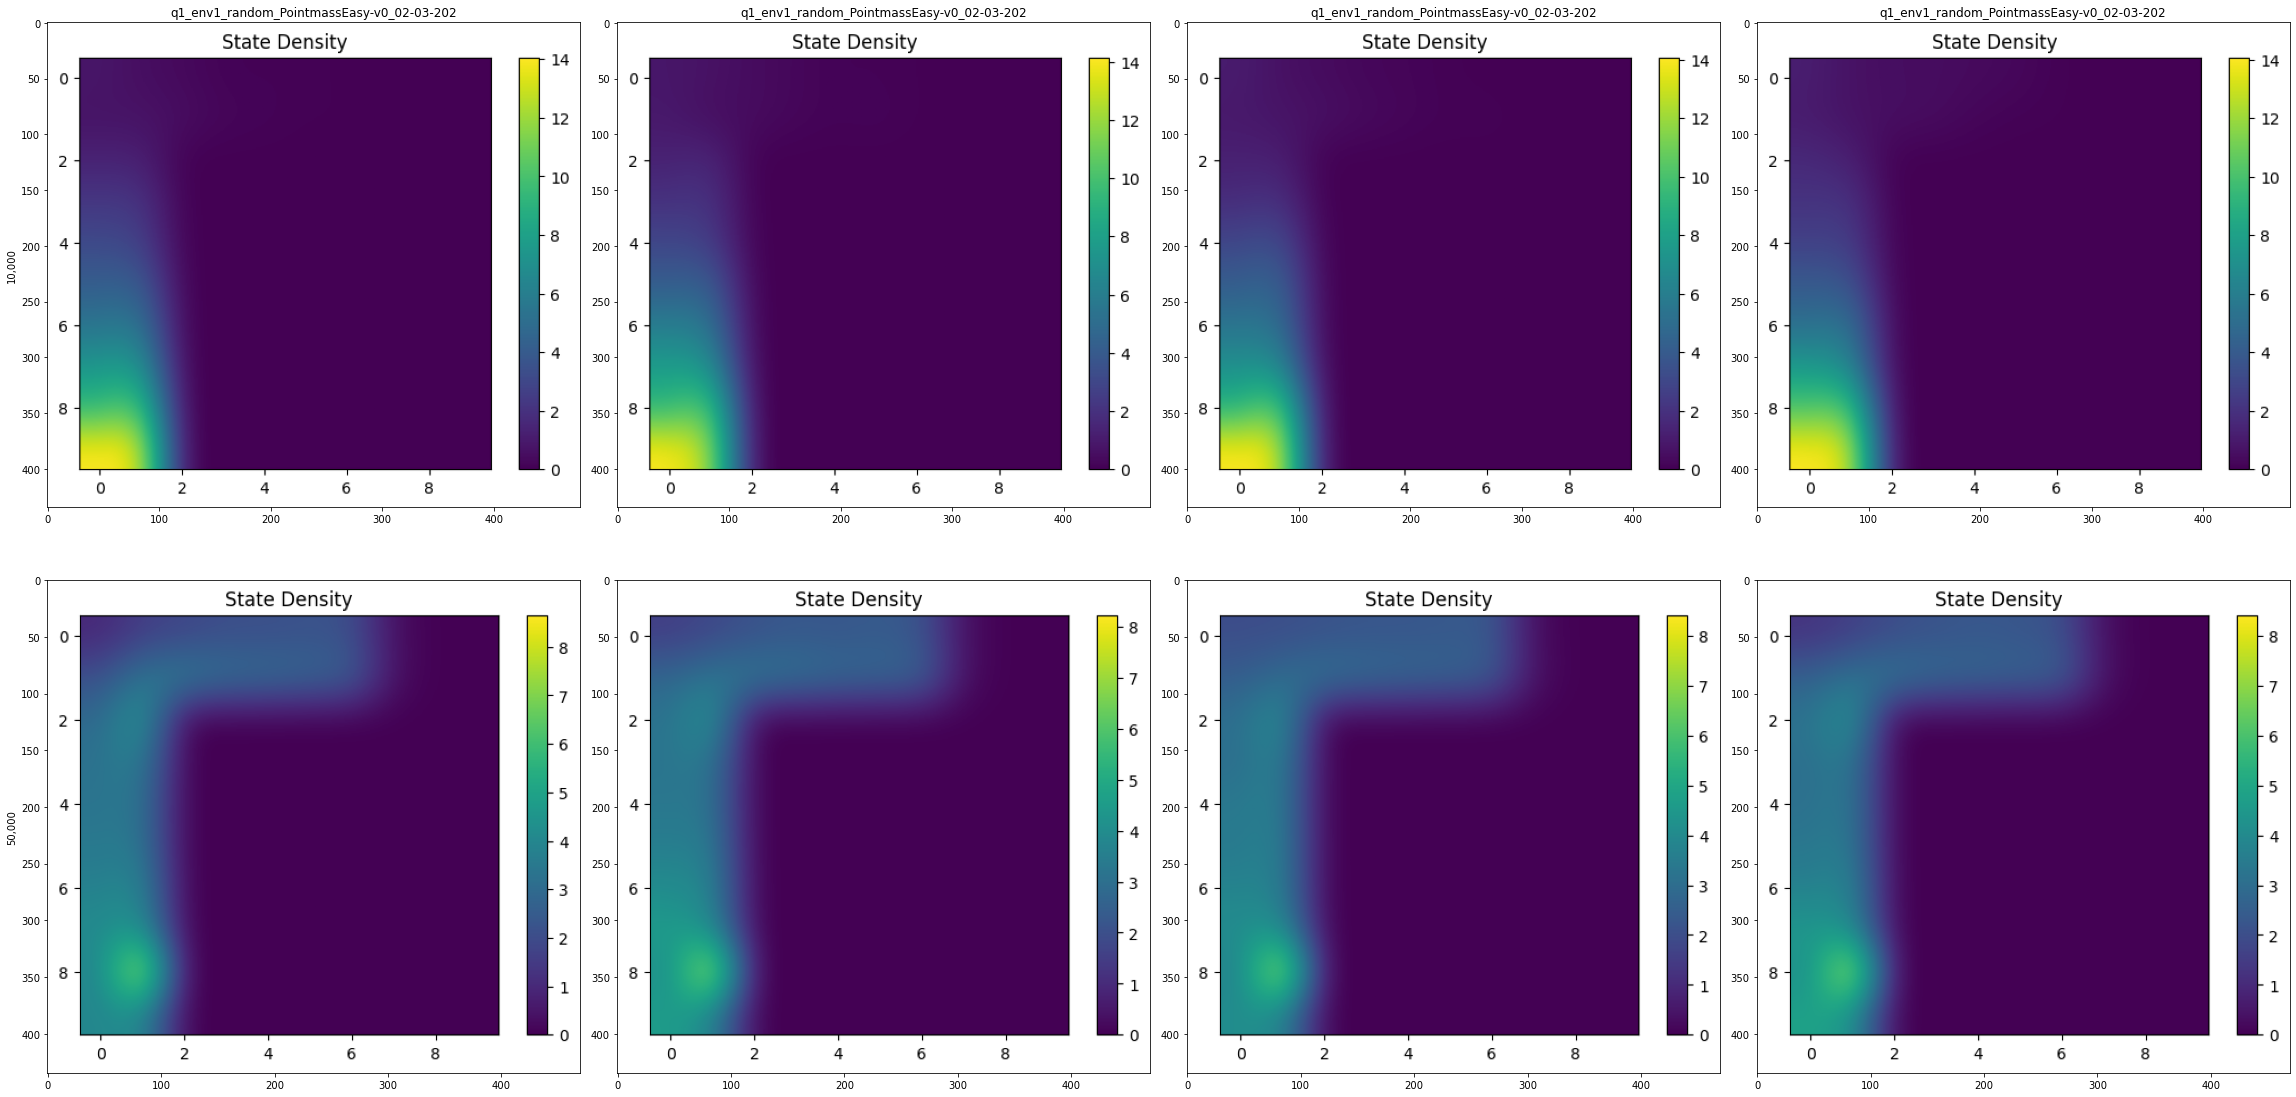
\includegraphics[scale=0.25]{q1/q1-easy-state-density-random}

    After 10K training steps, state density for the random strategy seems to be concentrated around the starting state and fades away as it moves away from the starting state.
    This is compatible with the expectation.

    \hspace*{-0.6in}
    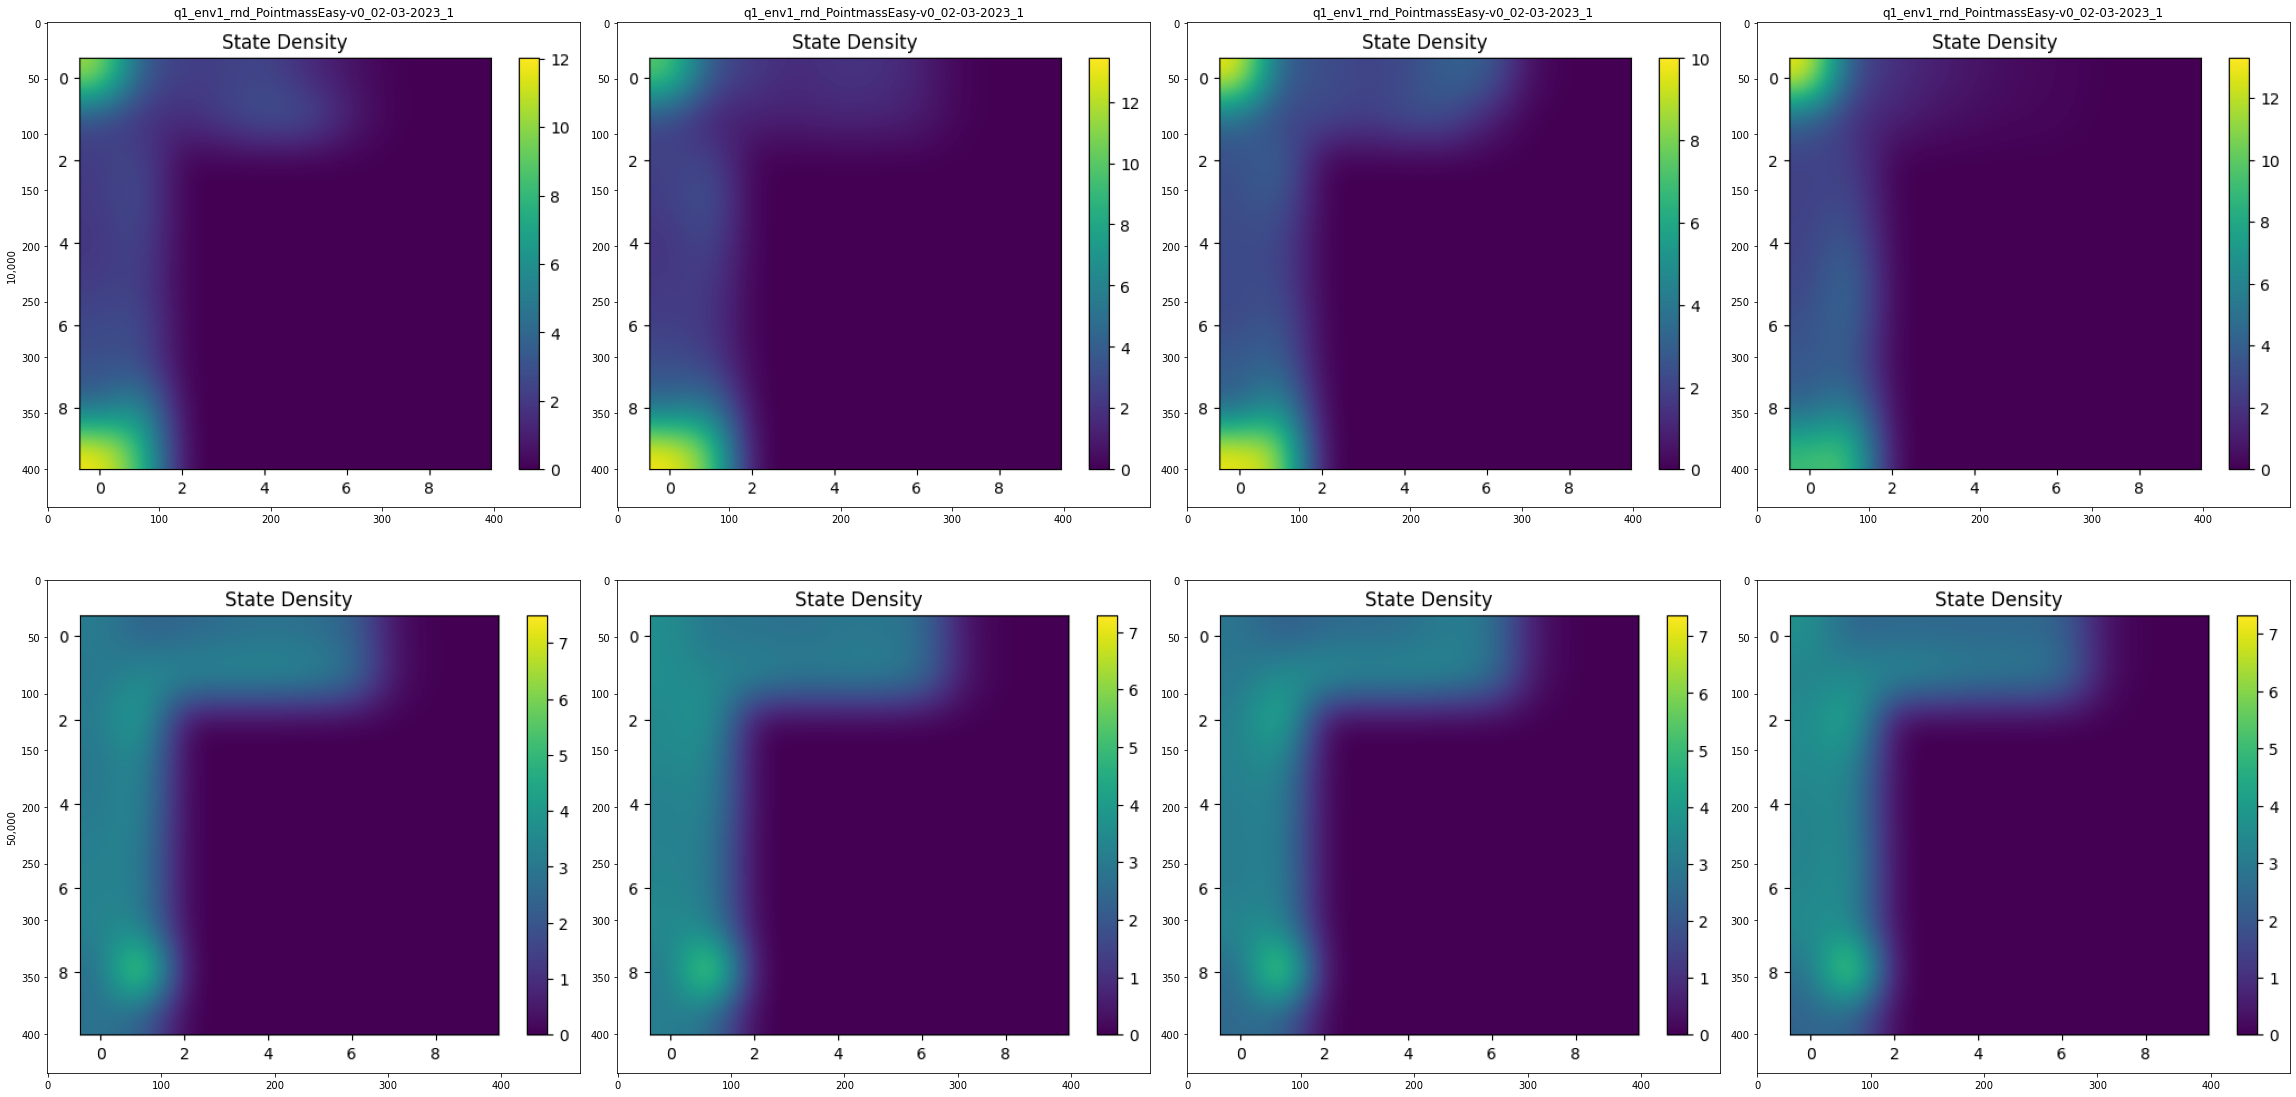
\includegraphics[scale=0.25]{q1/q1-easy-state-density-rnd}

    After 10K training steps, state density for the RND strategy seems to be more uniformly spread over the reachable parts of the environment.

    This is compatible with the expectation.

    However, RND strategy also shows concentrations, especially around top left corner.
    Why this is the case?
    After 3K steps, RND values for the reachable parts becomes zero or close to zero, it is not distinguishable by just looking at the plots.
    After this point exploration critic values tend to diminish.
    Remaining exploration critic values are not good enough to produce uniform transitions.
    The agent gets trapped around points where actions have similar exploration bonuses.
    This is the same situation as random exploration.

    Why the top left corner then?
    Because it is the only corner in the environment.
    Why diminishing exploration values favor corners, it is not very clear.

    After the online exploitation starts, state density becomes uniform over time.
    The difference between the two strategies disappears.

    \subsubsection*{Revisiting raining return}

    RND strategy exploration critic return reaches -30 then drops.
    The drop can be credited to fading exploration bonuses which is a result of diminished RDN values.
    Once exploitation starts, RND strategy has a somewhat decent exploitation critic which has been trained for 8K steps.
    Exploitation and training starts at the same time for the RND strategy.
    But it catch-ups after roughly 8K steps.
    In the easy environment RND strategy offers no advantage over the Random strategy.

    \hspace*{-0.6in}
    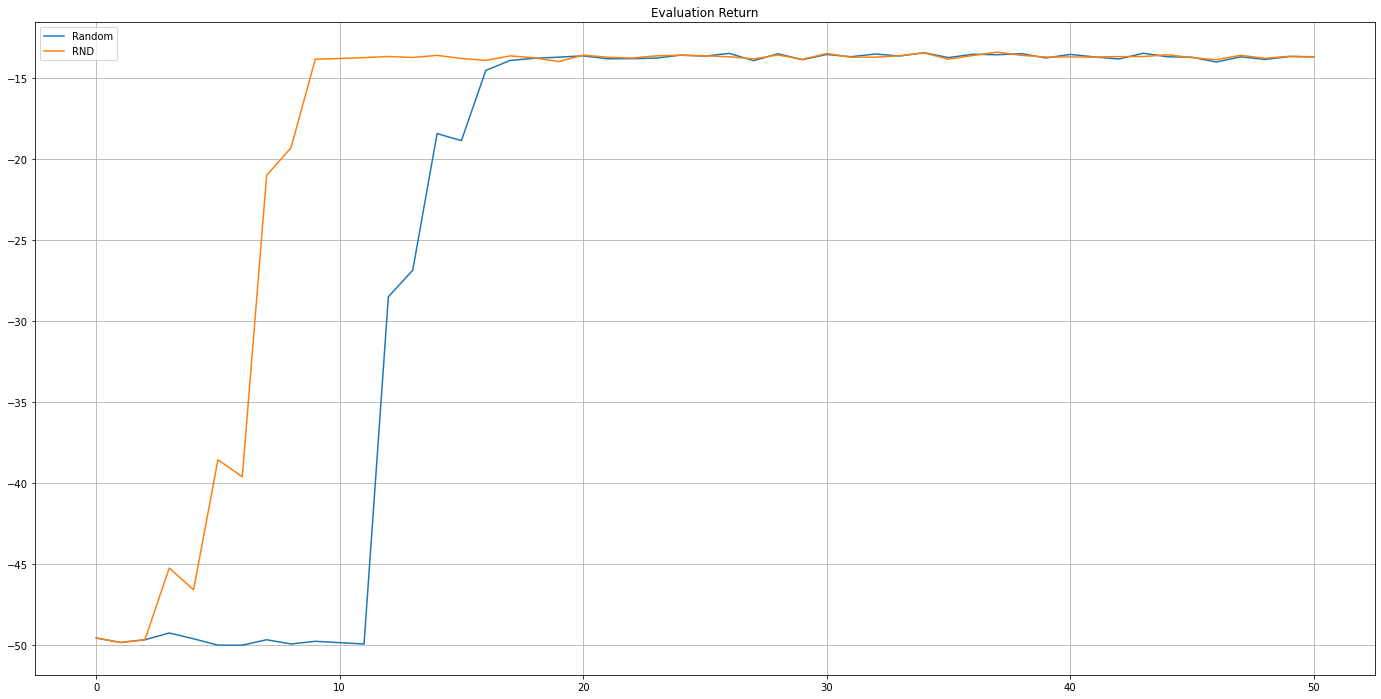
\includegraphics[scale=0.30]{q1/q1-easy-eval-compare}

    In terms of evaluation performance, both strategies perform the same.
    Note that random strategy starts learning after 10K steps while RND strategy starts learning after 2K steps.

    \subsubsection*{Medium Environment}

    \hspace*{-0.6in}
    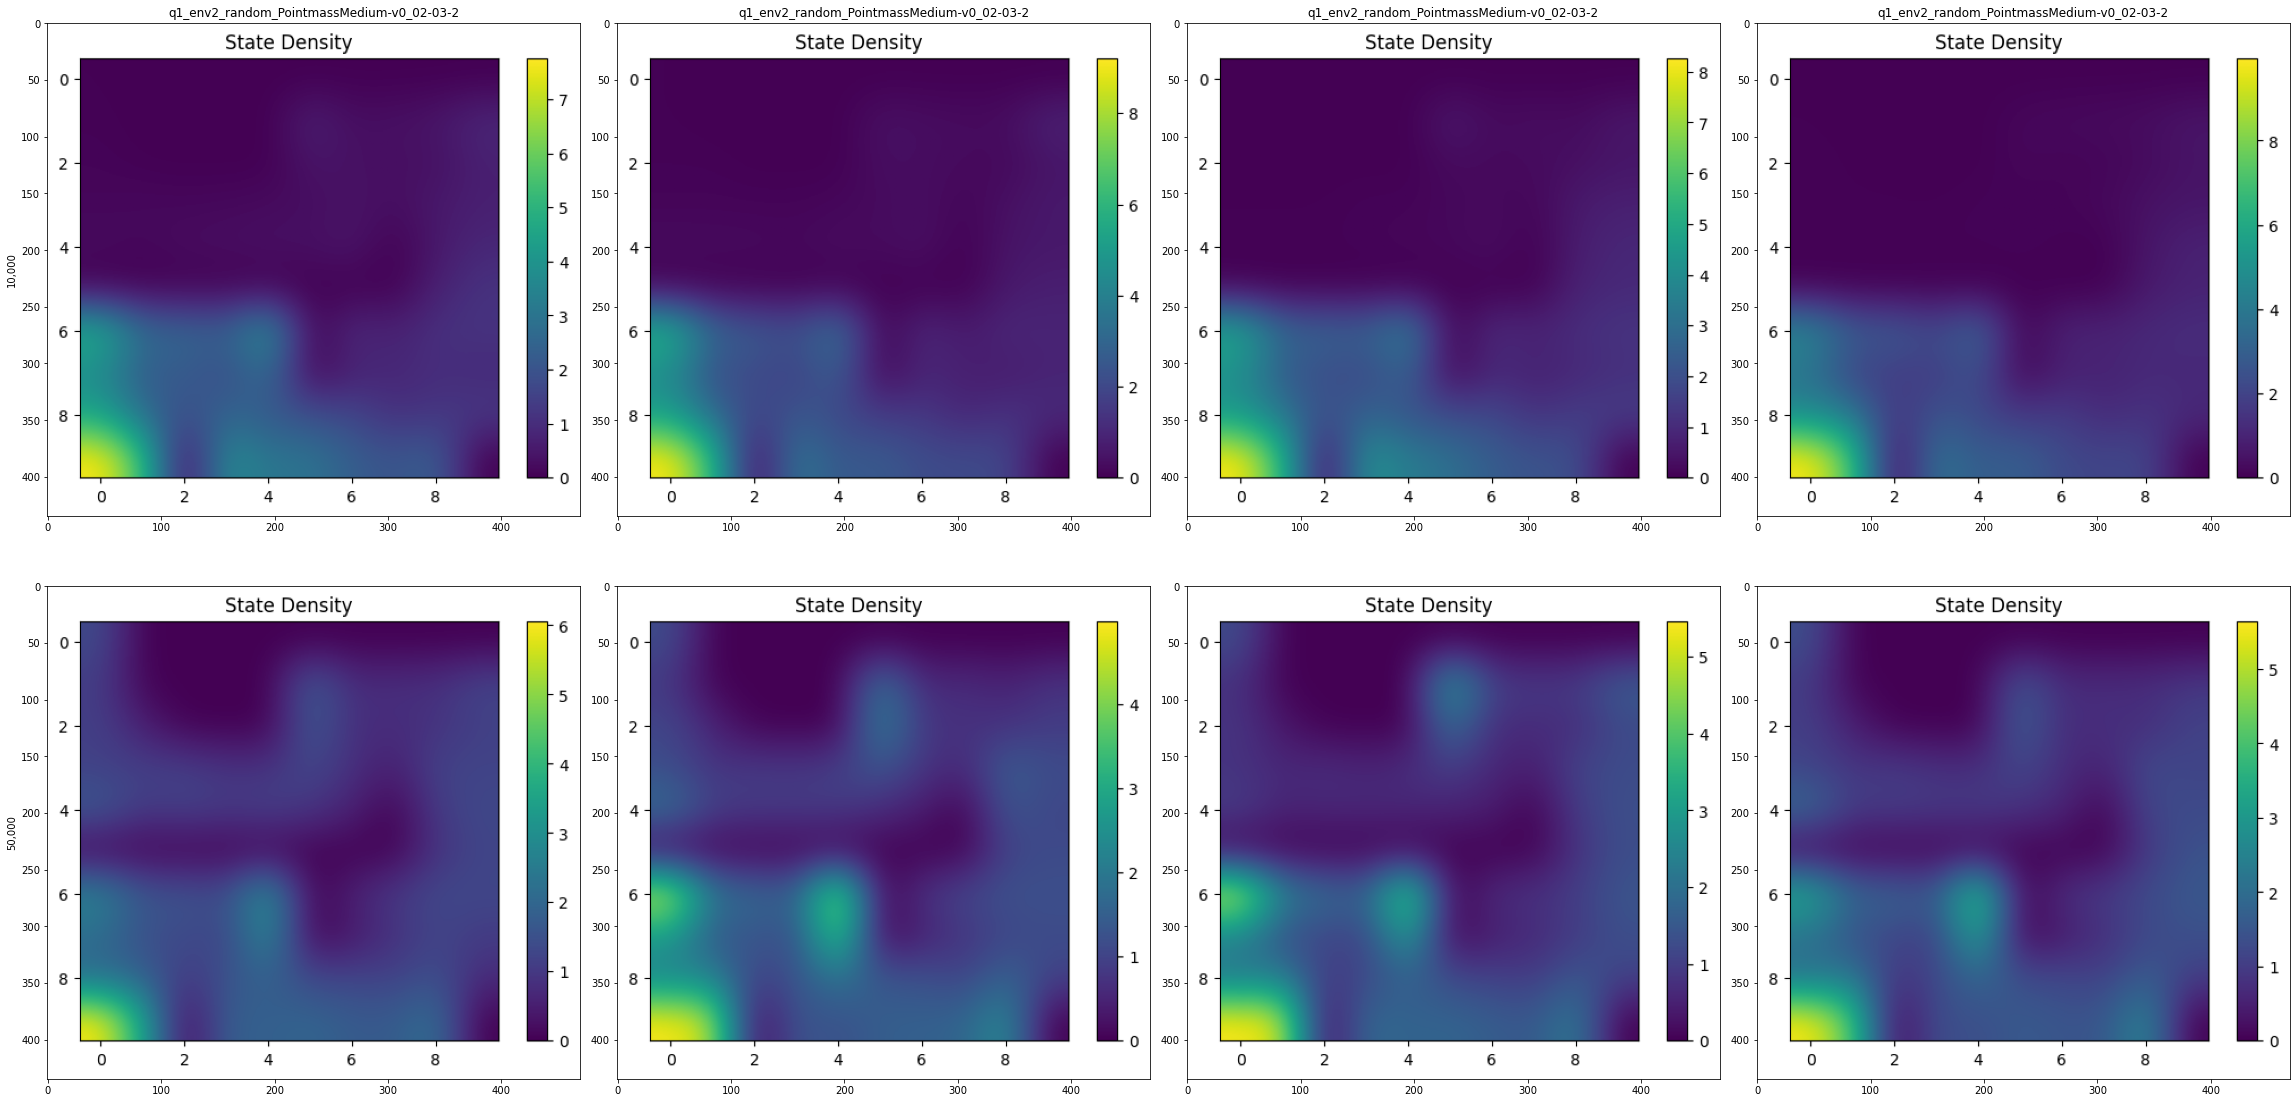
\includegraphics[scale=0.25]{q1/q1-medium-state-density-random}

    \hspace*{-0.6in}
    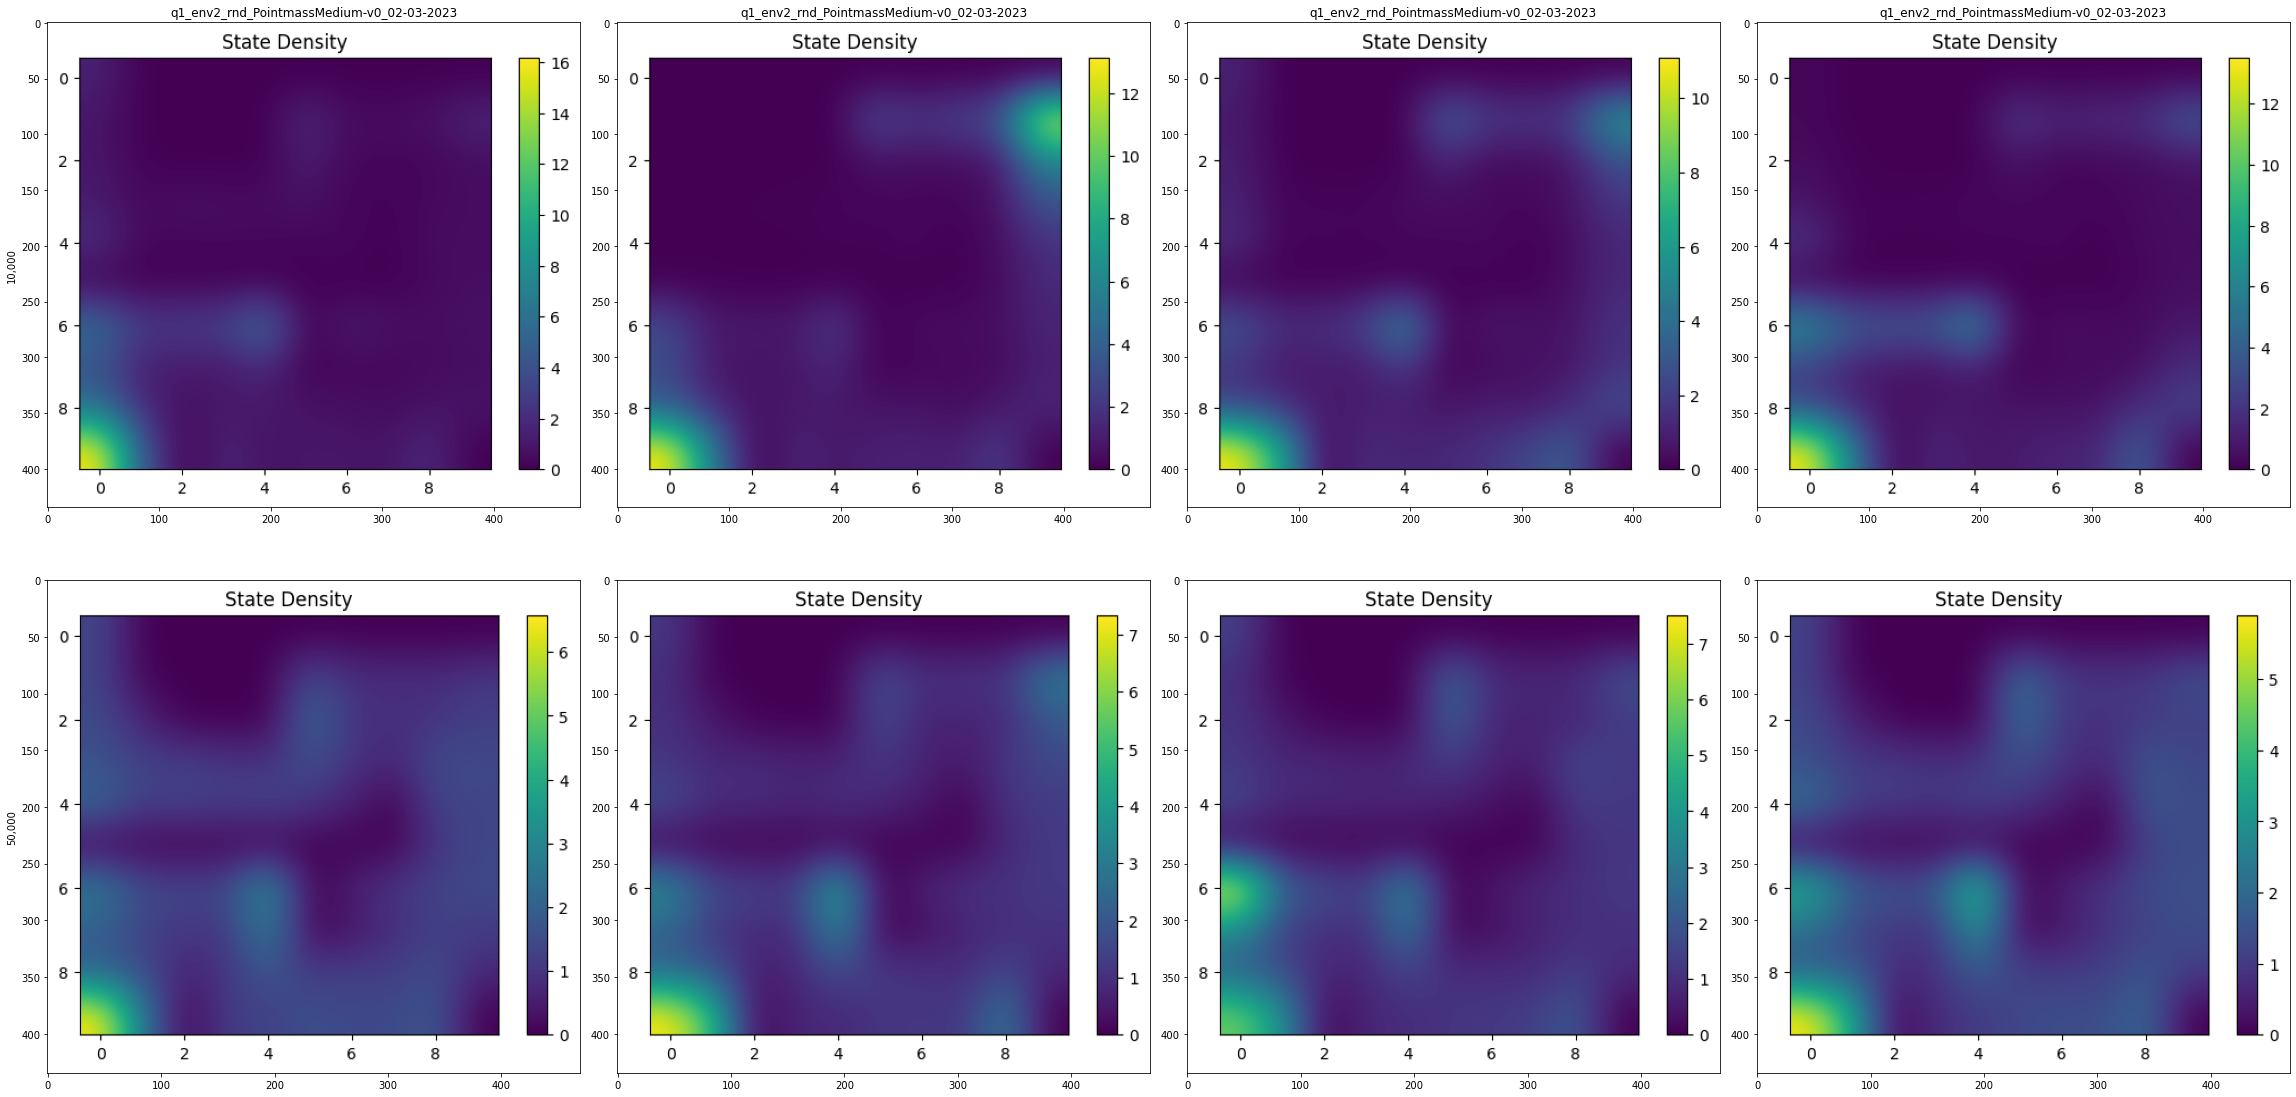
\includegraphics[scale=0.25]{q1/q1-medium-state-density-rnd}

    Random strategy generates state densities that are concentrated around the start state.
    Random strategy states density drops steadily as distance to start state increases.
    This behaviour is expected.

    RND strategy is expected to generate more uniform state densities, which seems not to be the case.
    Even in the early 3K steps, generated state densities suffer from multi-modalities, e.g. there are 2-3 concentration points.
    This is an indication of a flat exploration critic surface.

    \hspace*{-0.6in}
    \includegraphics[scale=0.25]{q1/q1-medium-exploration-values-rnd}

    Investigating exploration values show that in the beginning center states happen to be assigned lower values.
    This prevents the agent from exploring further.

    \hspace*{-0.6in}
    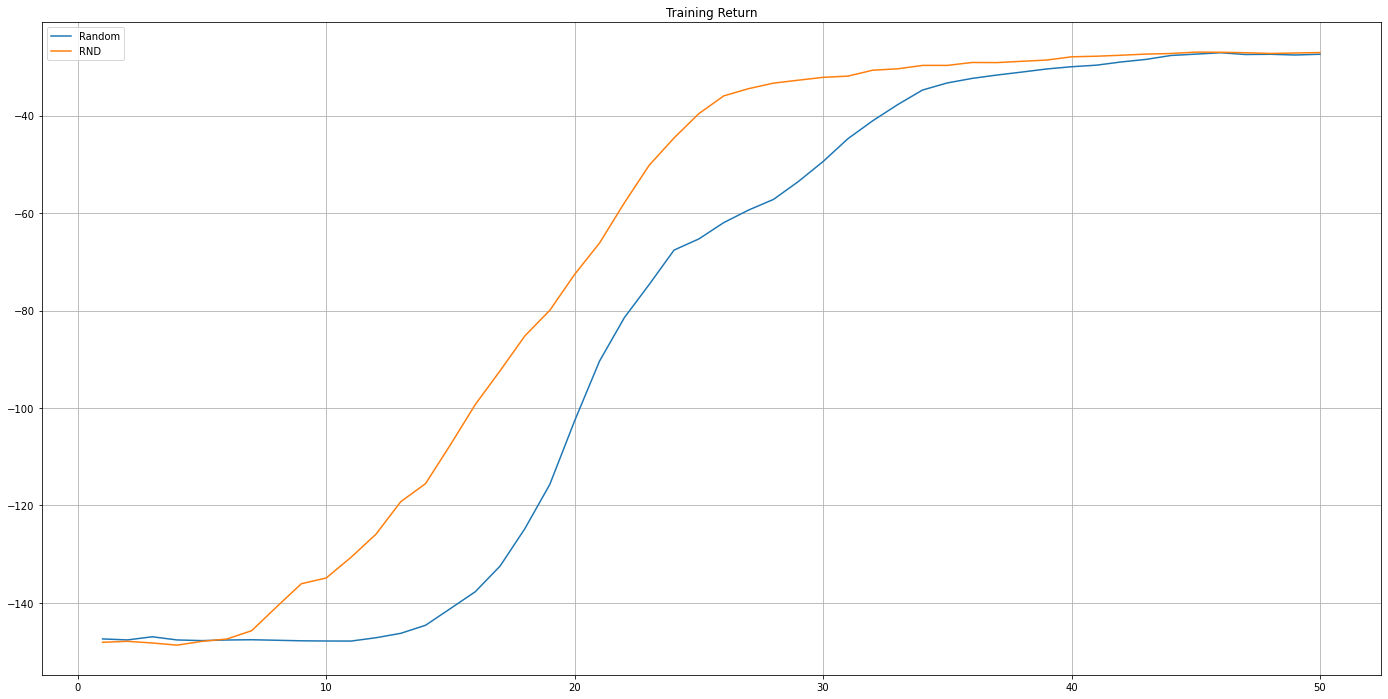
\includegraphics[scale=0.30]{q1/q1-medium-train-compare}

    RND strategy agent training average return starts rising after 10K steps, the point where exploiting agent takes on.
    8K steps training does not seem to pay off.
    Given the fact that exploration critic values are poor this is not surprising.

    Random strategy agent training average return starts rising after 15K steps.
    The curve is more steep than the RND curve.
    Also note that RND starts learning after 2K steps which means it has a 8K steps advantage.
    If Random strategy training curve started rising after 18K steps, we would argue that they behave similar, but actually by rising after 15K steps random strategy performs better.

    However, around 22K steps, while the gap was about to close, Random training curve takes a hit and levels out.
    It is only around 50K steps that the Random strategy can catches-up again.
    This hit is not expected.

    Remember that after exploitation starts both strategies continues with epsilon greedy exploration.
    So called Random strategy already has a better critic which makes it learn faster.
    At this point Random agent has nothing to make him perform inferior.

    \hspace*{-0.6in}
    \includegraphics[scale=0.9]{q1/q1-medium-train-compare-seeds}

    It is necessary to investigate training performance for each seed to understand what actually is going on.

    Please ignore the leading 0 in the plots.

    It turns out one of the Random strategy experiments performs very poorly and impacts the overall average performance values.
    If the unlucky seed is left out Random strategy average becomes better than the RND.

    This observation can be used to argue that RND strategy is more robust, but there is not enough evidence to support this.

    \hspace*{-0.6in}
    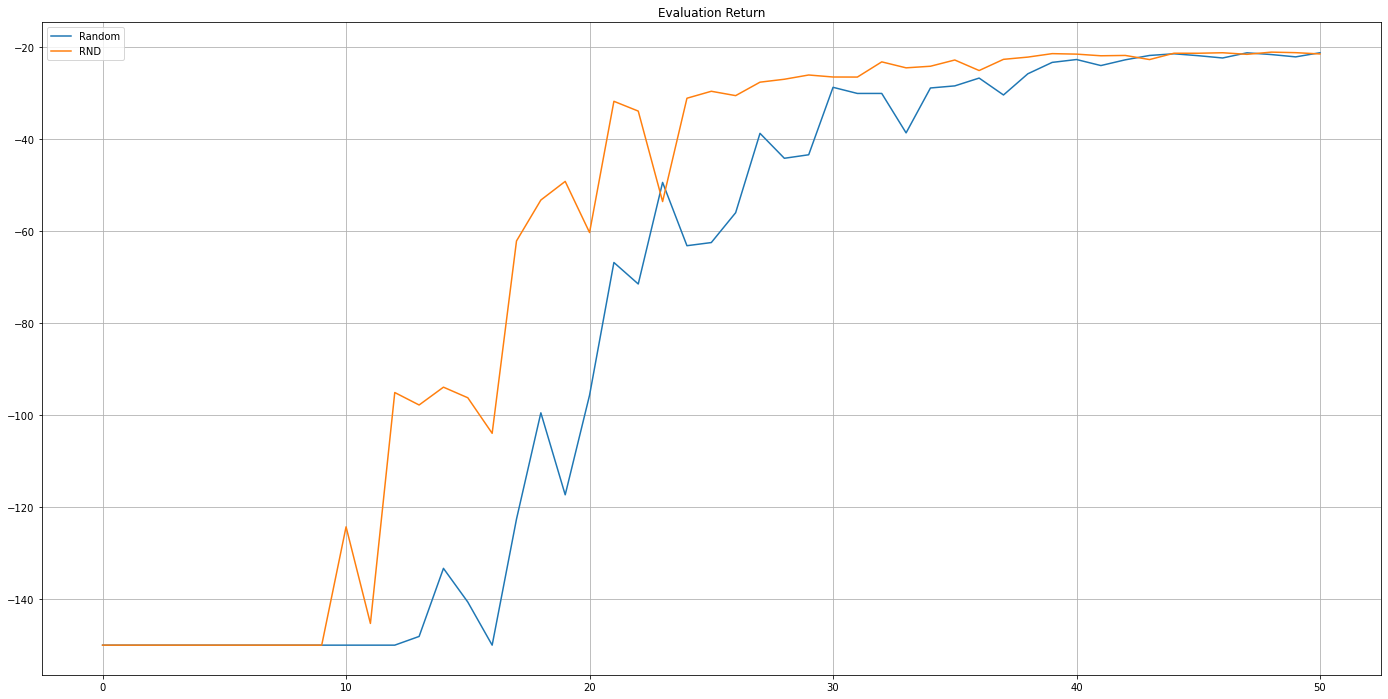
\includegraphics[scale=0.30]{q1/q1-medium-eval-compare}

    Evaluation performance follows the same discussions made for the training performance.
    One slight difference to note is RND exploitation critic gives rise to evaluation returns after training starts, in comparison to training curve.

    \subsubsection*{Hard Environment}

    \hspace*{-0.6in}
    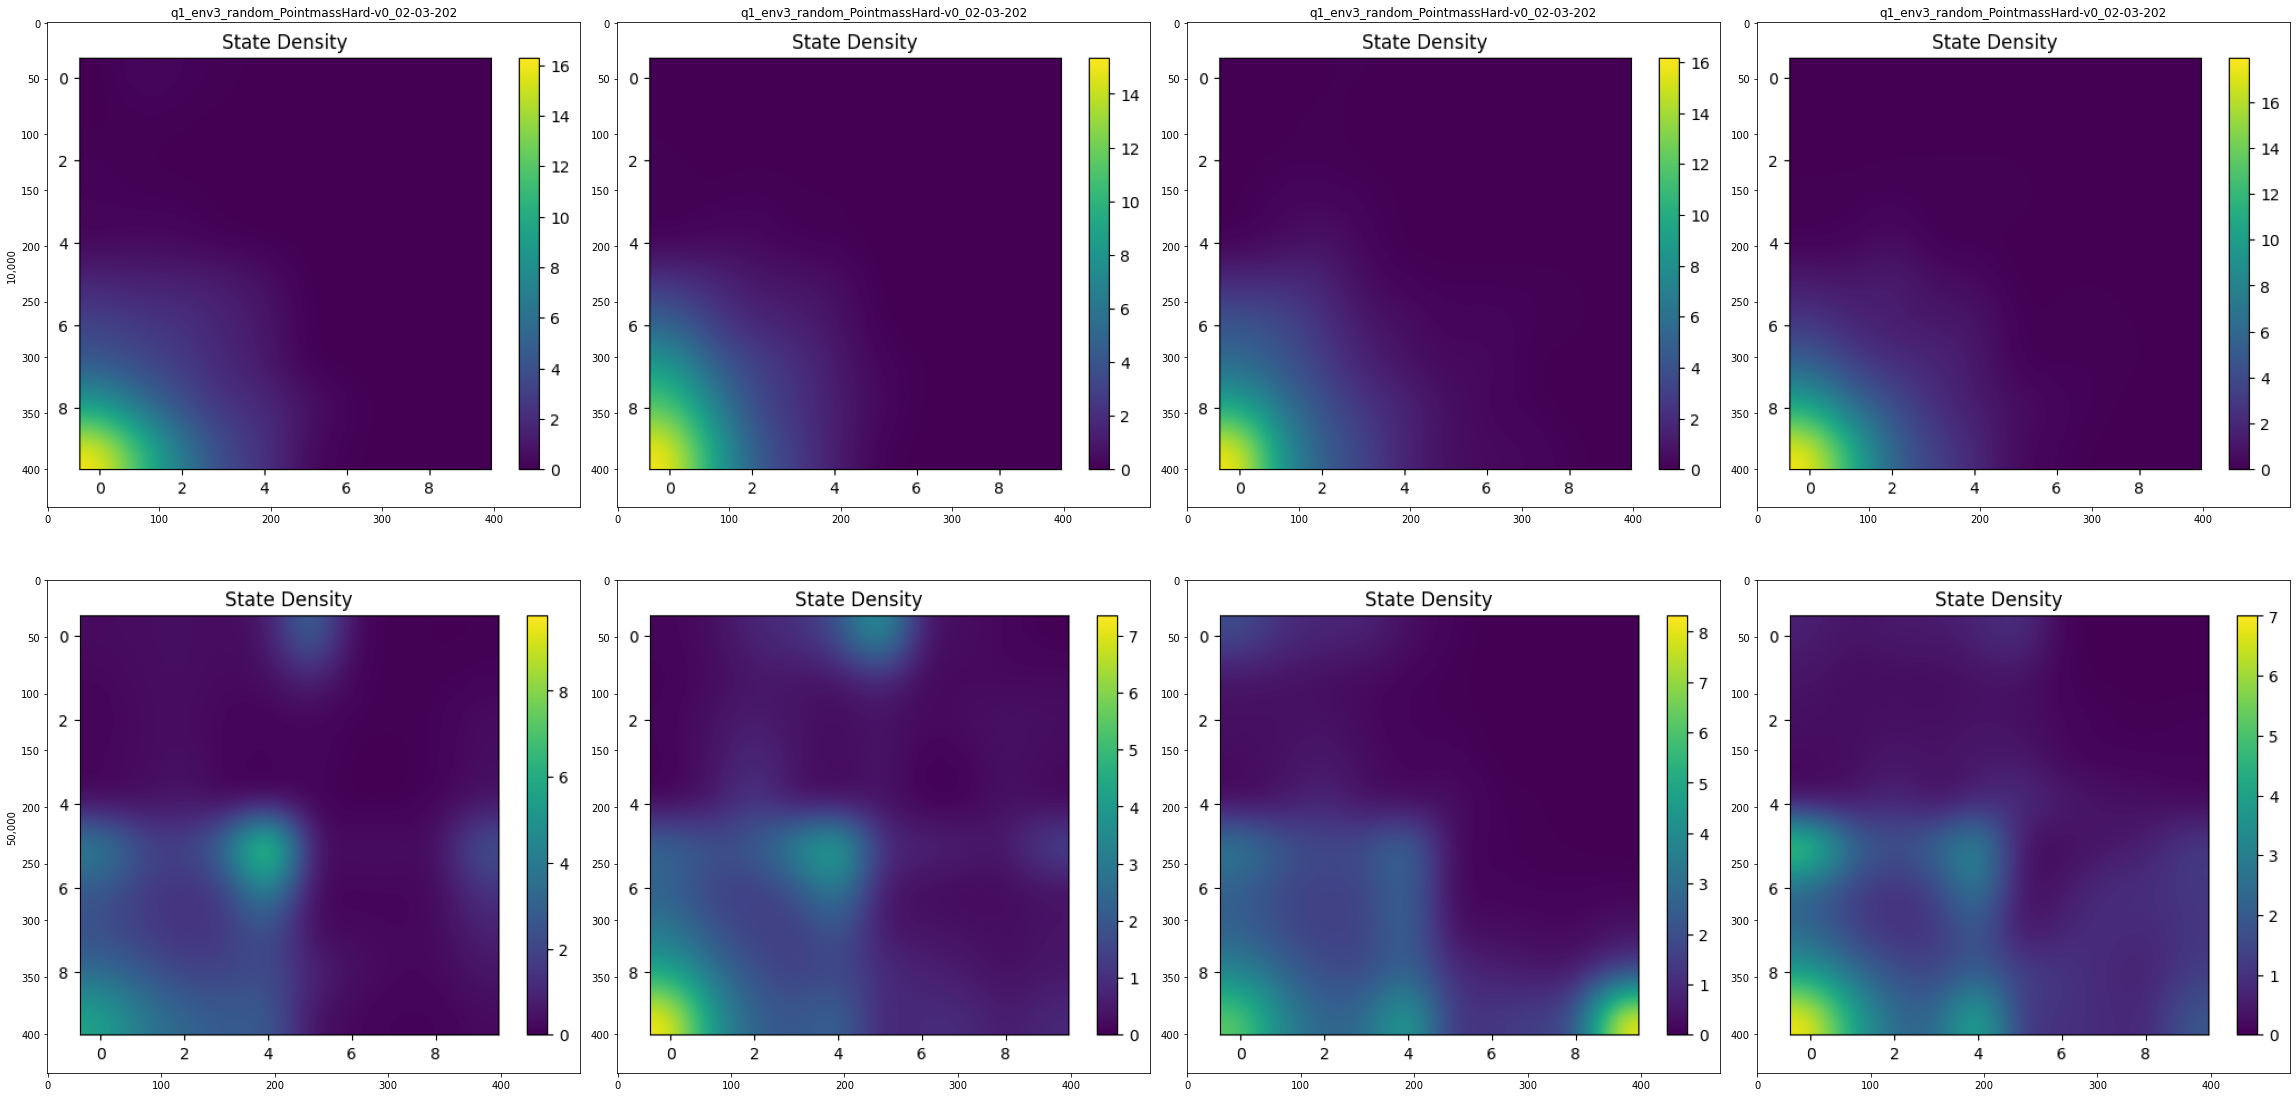
\includegraphics[scale=0.25]{q1/q1-hard-state-density-random}

    \hspace*{-0.6in}
    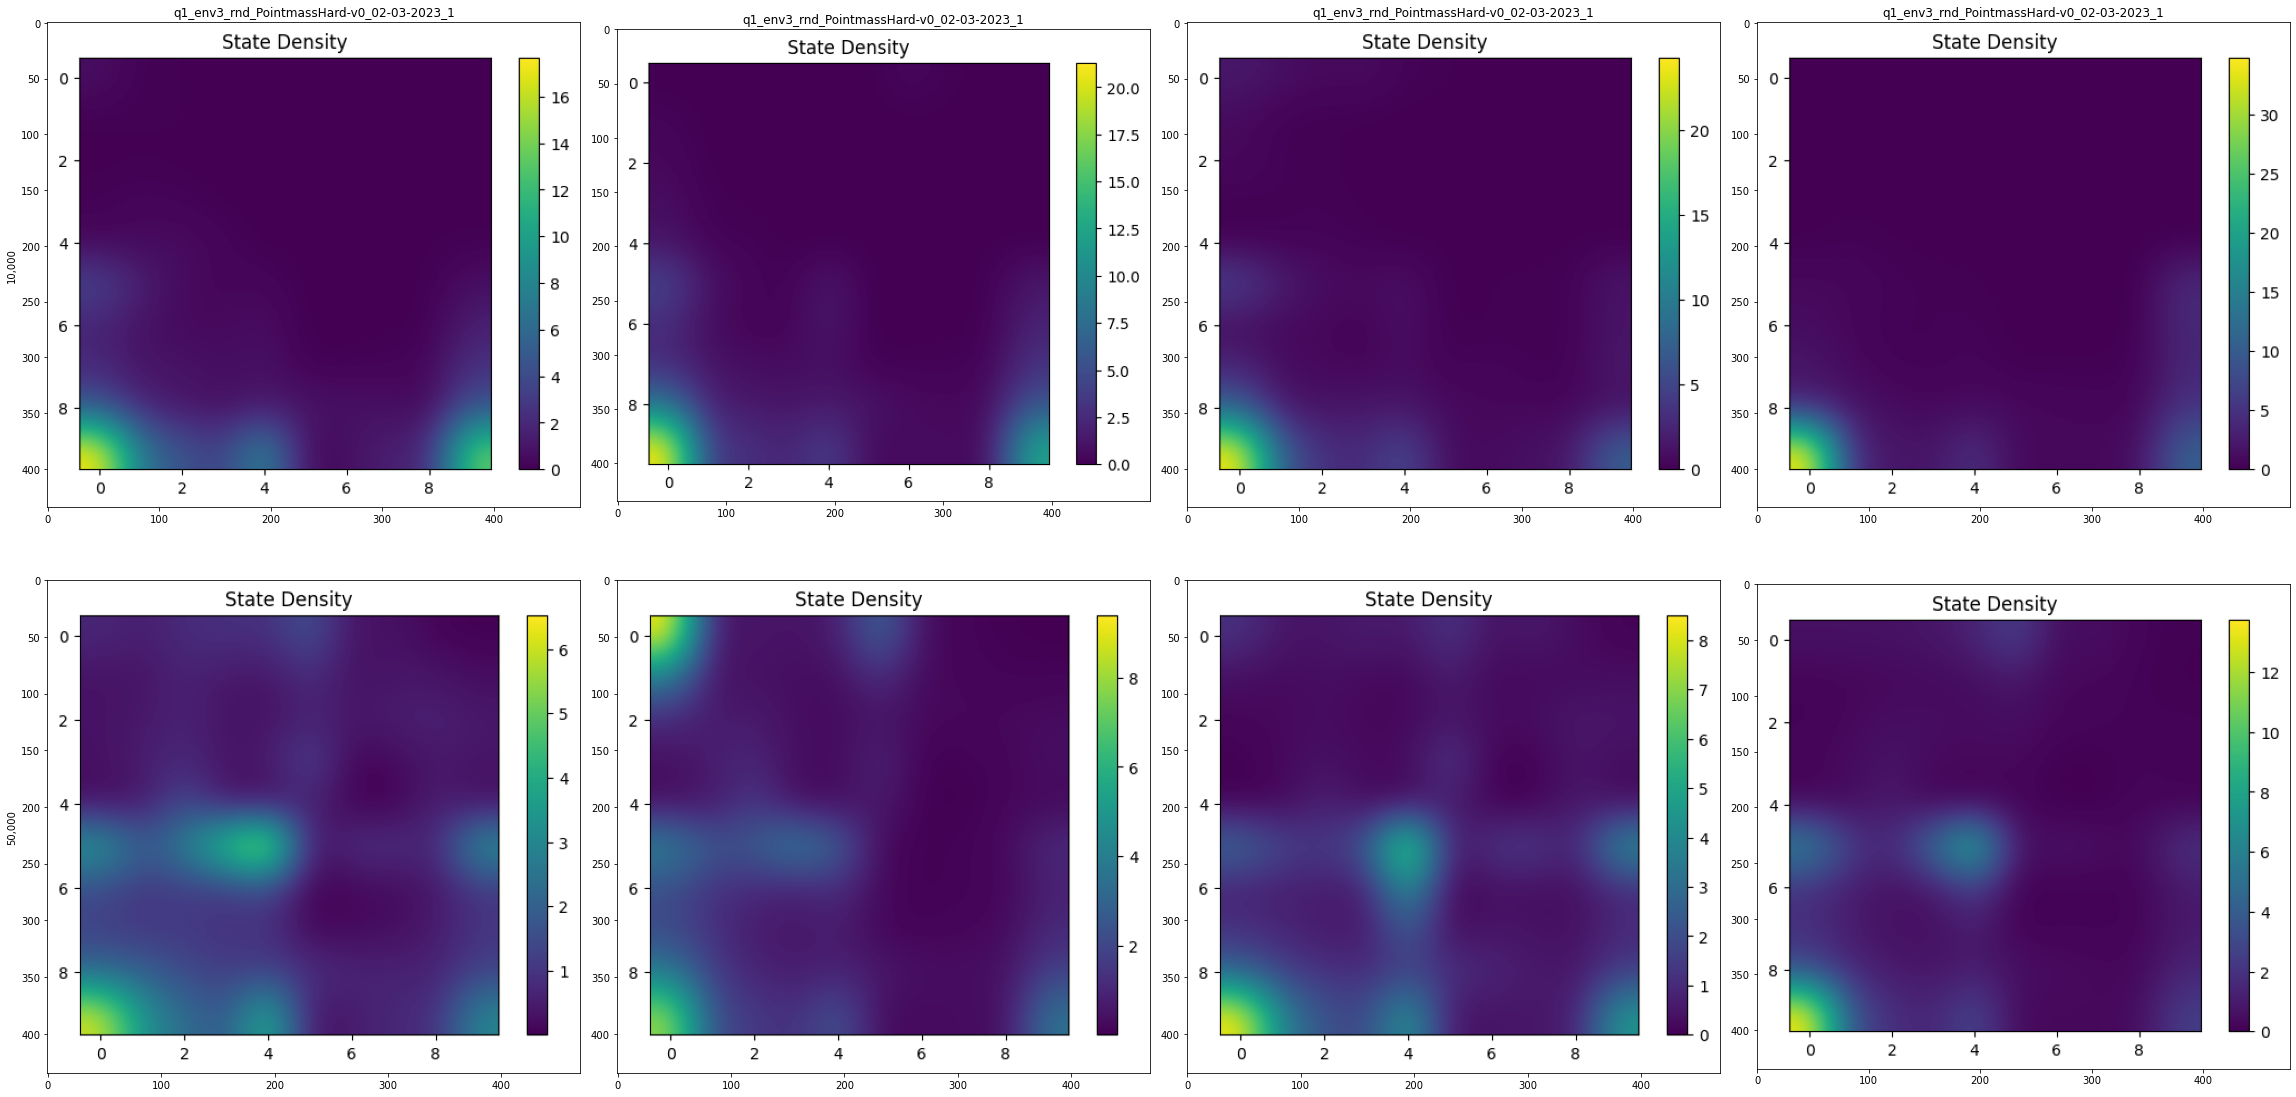
\includegraphics[scale=0.25]{q1/q1-hard-state-density-rnd}

    Random strategy explores only the first room.
    It fails to reach the other rooms.

    RND strategy has a clear advantage in the hard environment.

    \hspace*{-0.6in}
    \includegraphics[scale=0.30]{q1/q1-hard-train-10k-merge-traj-random}

    \hspace*{-0.6in}
    \includegraphics[scale=0.30]{q1/q1-hard-train-10k-merge-traj-rnd}

    Training trajectory images are collected and merged together to generate a density of training trajectories.
    Only first 10K trajectories are used.
    Note that this aggregate images are similar to state densities but different in that they add the lines between points as well so that they are more clear and uses a trajectory only once instead of sampling.

    First image belongs to random strategy experiments.
    The second image belongs to rnd strategy experiments.
    Exploration superiority of the RND strategy is clear.

    \hspace*{-0.6in}
    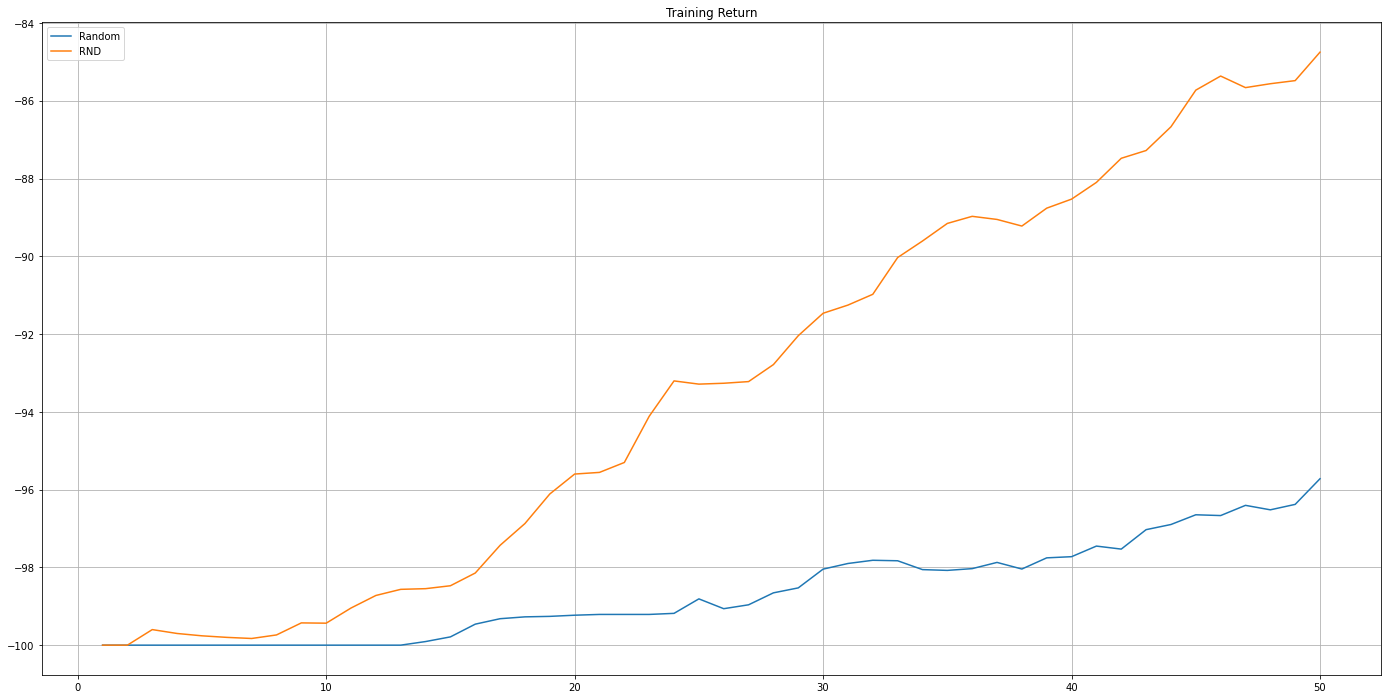
\includegraphics[scale=0.30]{q1/q1-hard-train-compare}

    \hspace*{-0.6in}
    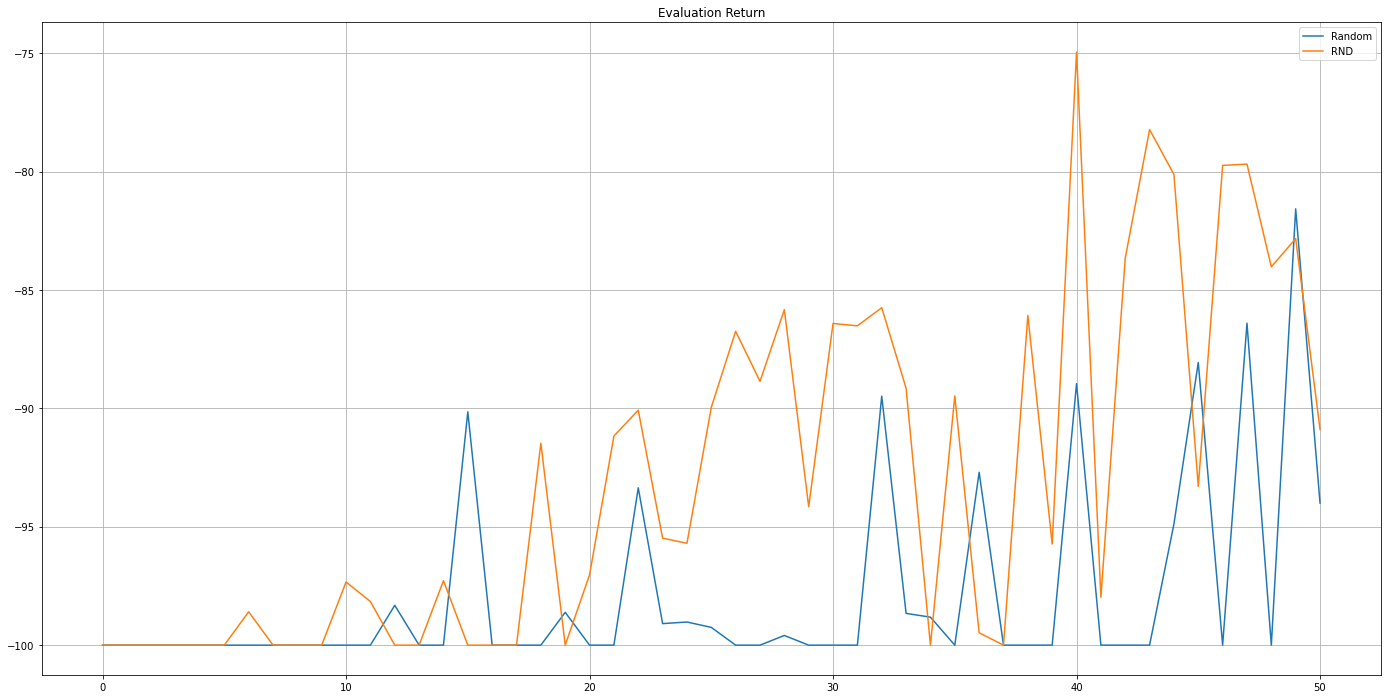
\includegraphics[scale=0.30]{q1/q1-hard-eval-compare}

    Random strategy training performance is poor because it fails to explore properly.

    RND strategy on the other hand makes use of the critic values learned during exploration.
    The gap between RND and random strategy performances keeps open rather than closing as it was the in case in the previous environments.


    \subsection*{Count Based Exploration Implementation}

    Target environment is a simple 2D environment.
    A simple count based exploration strategy can be used.

    A state representation consists two features each in the range of 0-1.
    State aggregation can be used to decrease number of states.
    0-1 range is discretized into 50 parts.
    Counts are kept in the discretized space.
    Count table consists of 2500 elements.
    Each table element is initialized to 1.

    Count based exploration strategy is implemented in a similar way to RND strategy.
    So results are expected to be at least as good as RND strategy.

    During training, state S is discretized into s.
    At each training step count for state s is increased by 1.
    Exploration bonus is calculated as 1/CNT(s) where CNT(s) gives the count for the discretized state s.

    Count based exploration strategy is referred to as CNT in the following discussions.

    \subsubsection*{Easy Environment}

    \hspace*{-0.6in}
    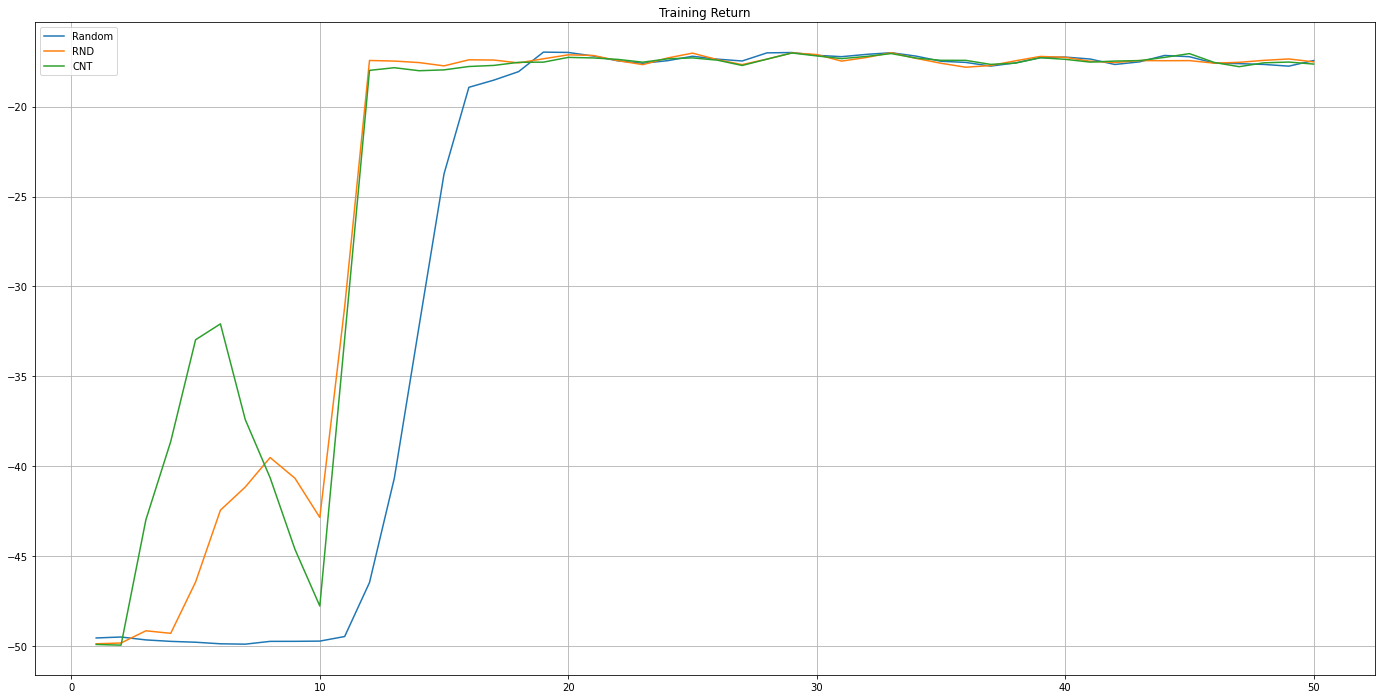
\includegraphics[scale=0.30]{q1/q1-p2-cnt-easy-train}

    \hspace*{-0.6in}
    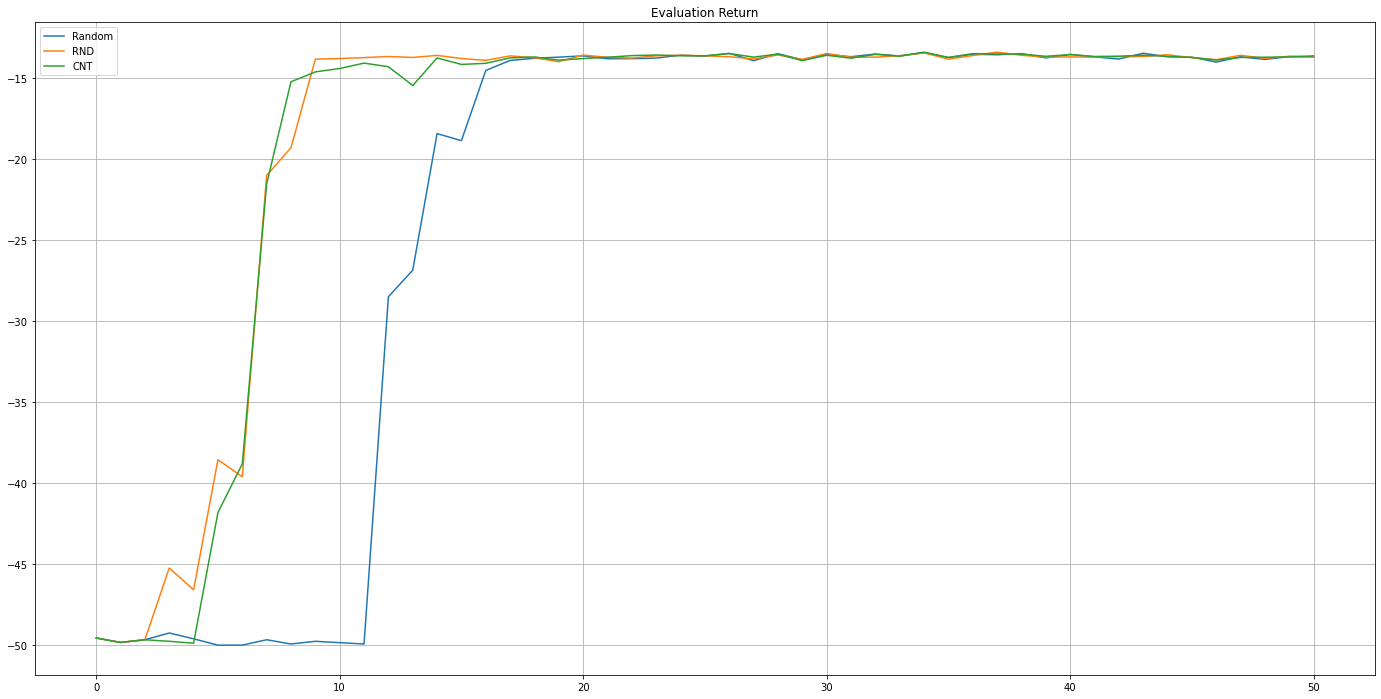
\includegraphics[scale=0.30]{q1/q1-p2-cnt-easy-eval}

    \hspace*{-0.6in}
    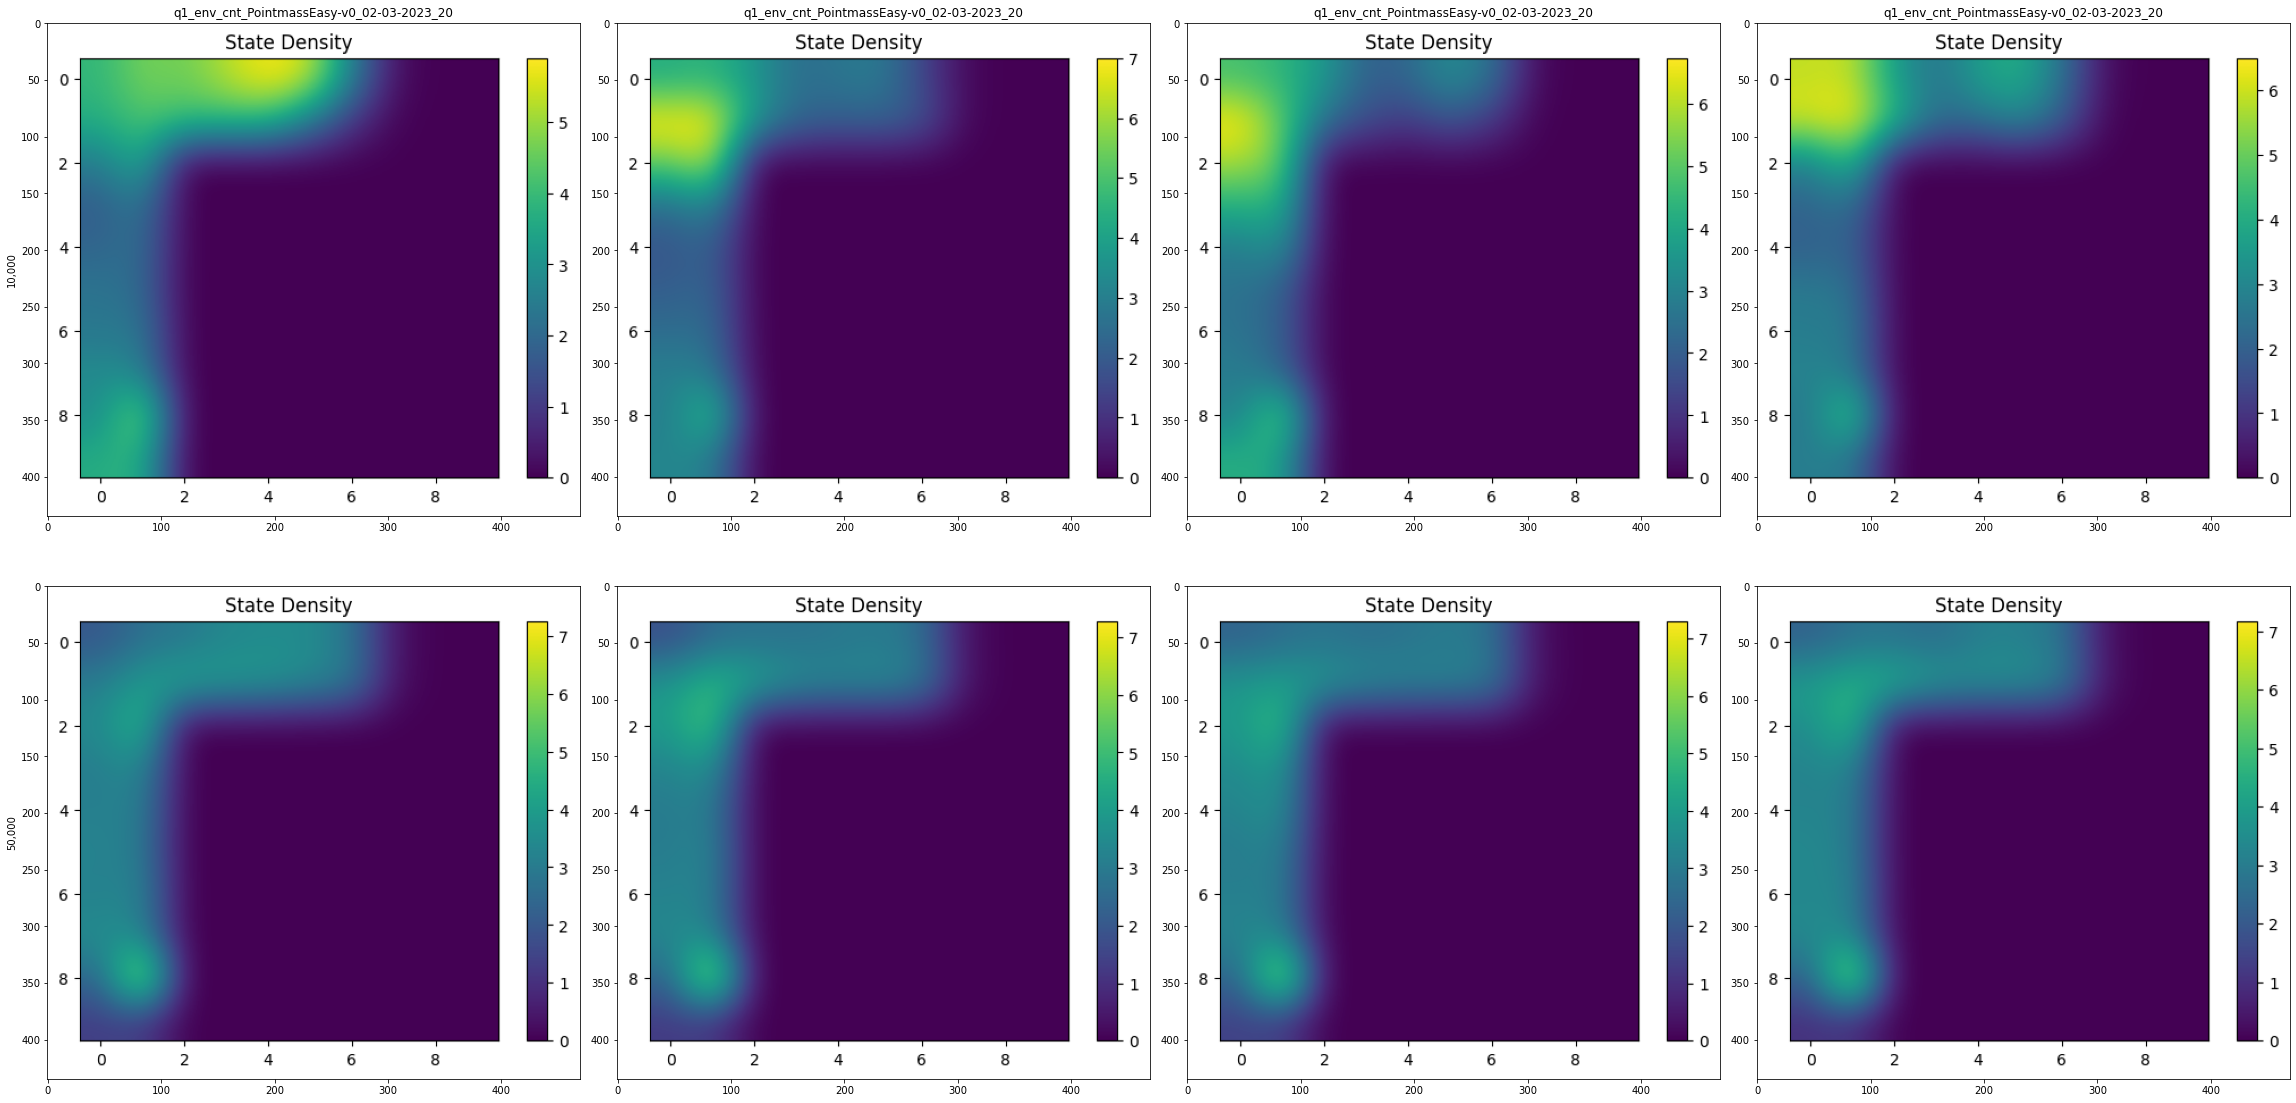
\includegraphics[scale=0.25]{q1/q1-p2-cnt-easy-state-density}

    Count based exploration strategy produces more uniform state density.
    In terms of training and evaluation performance CNT performs similar to RND strategy.
    In the easy environment difference is not distinguishable.

    \subsubsection*{Medium Environment}

    \hspace*{-0.6in}
    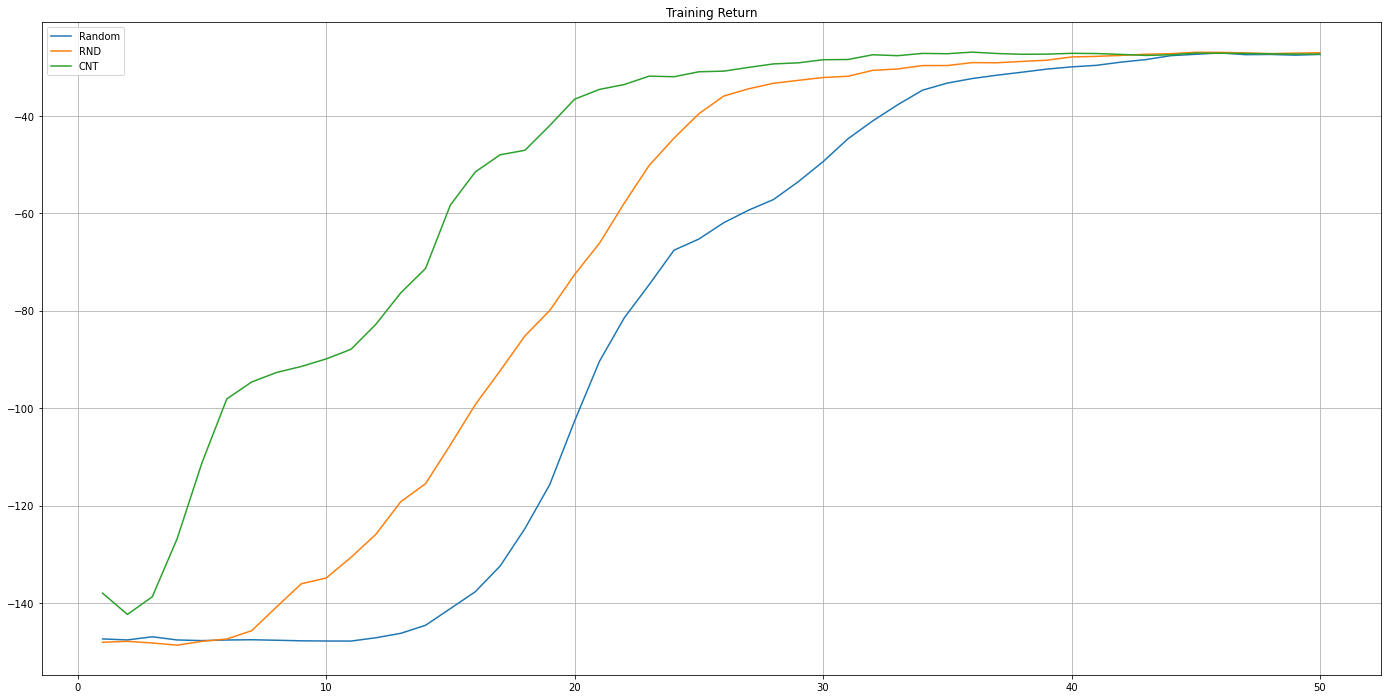
\includegraphics[scale=0.30]{q1/q1-p2-cnt-medium-train}

    \hspace*{-0.6in}
    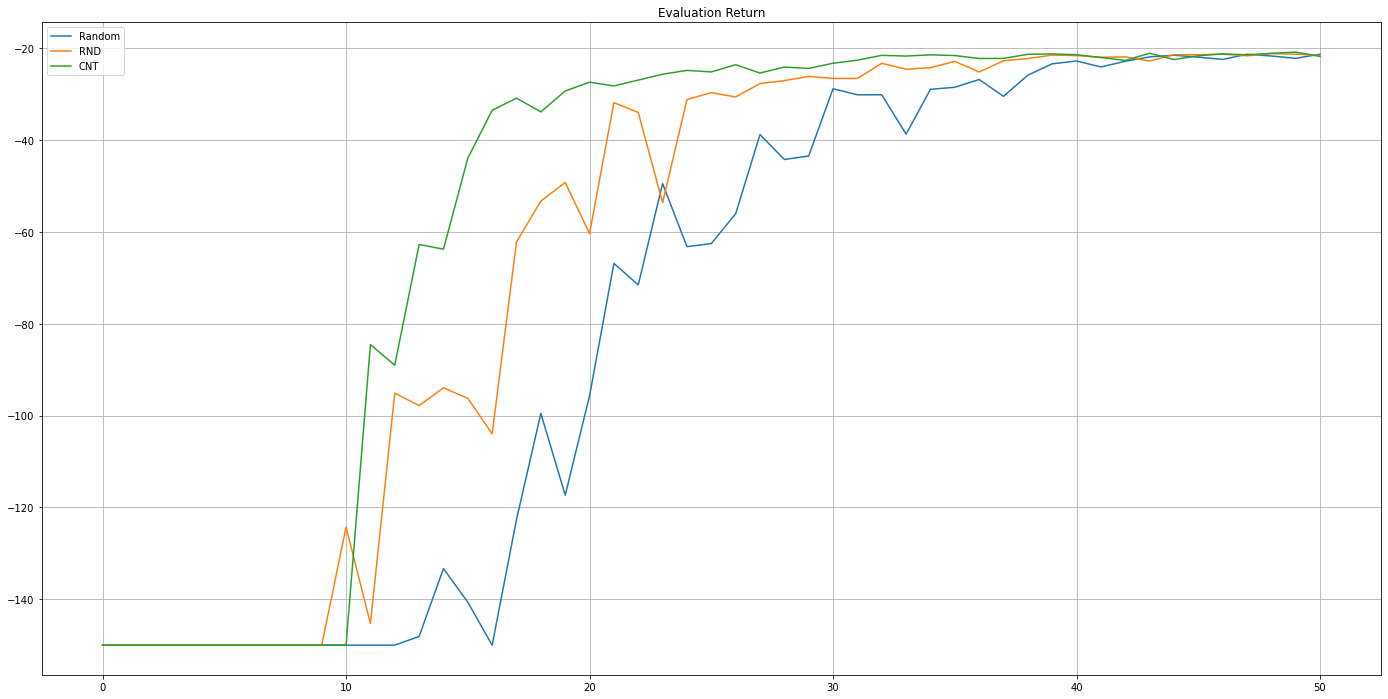
\includegraphics[scale=0.30]{q1/q1-p2-cnt-medium-eval}

    \hspace*{-0.6in}
    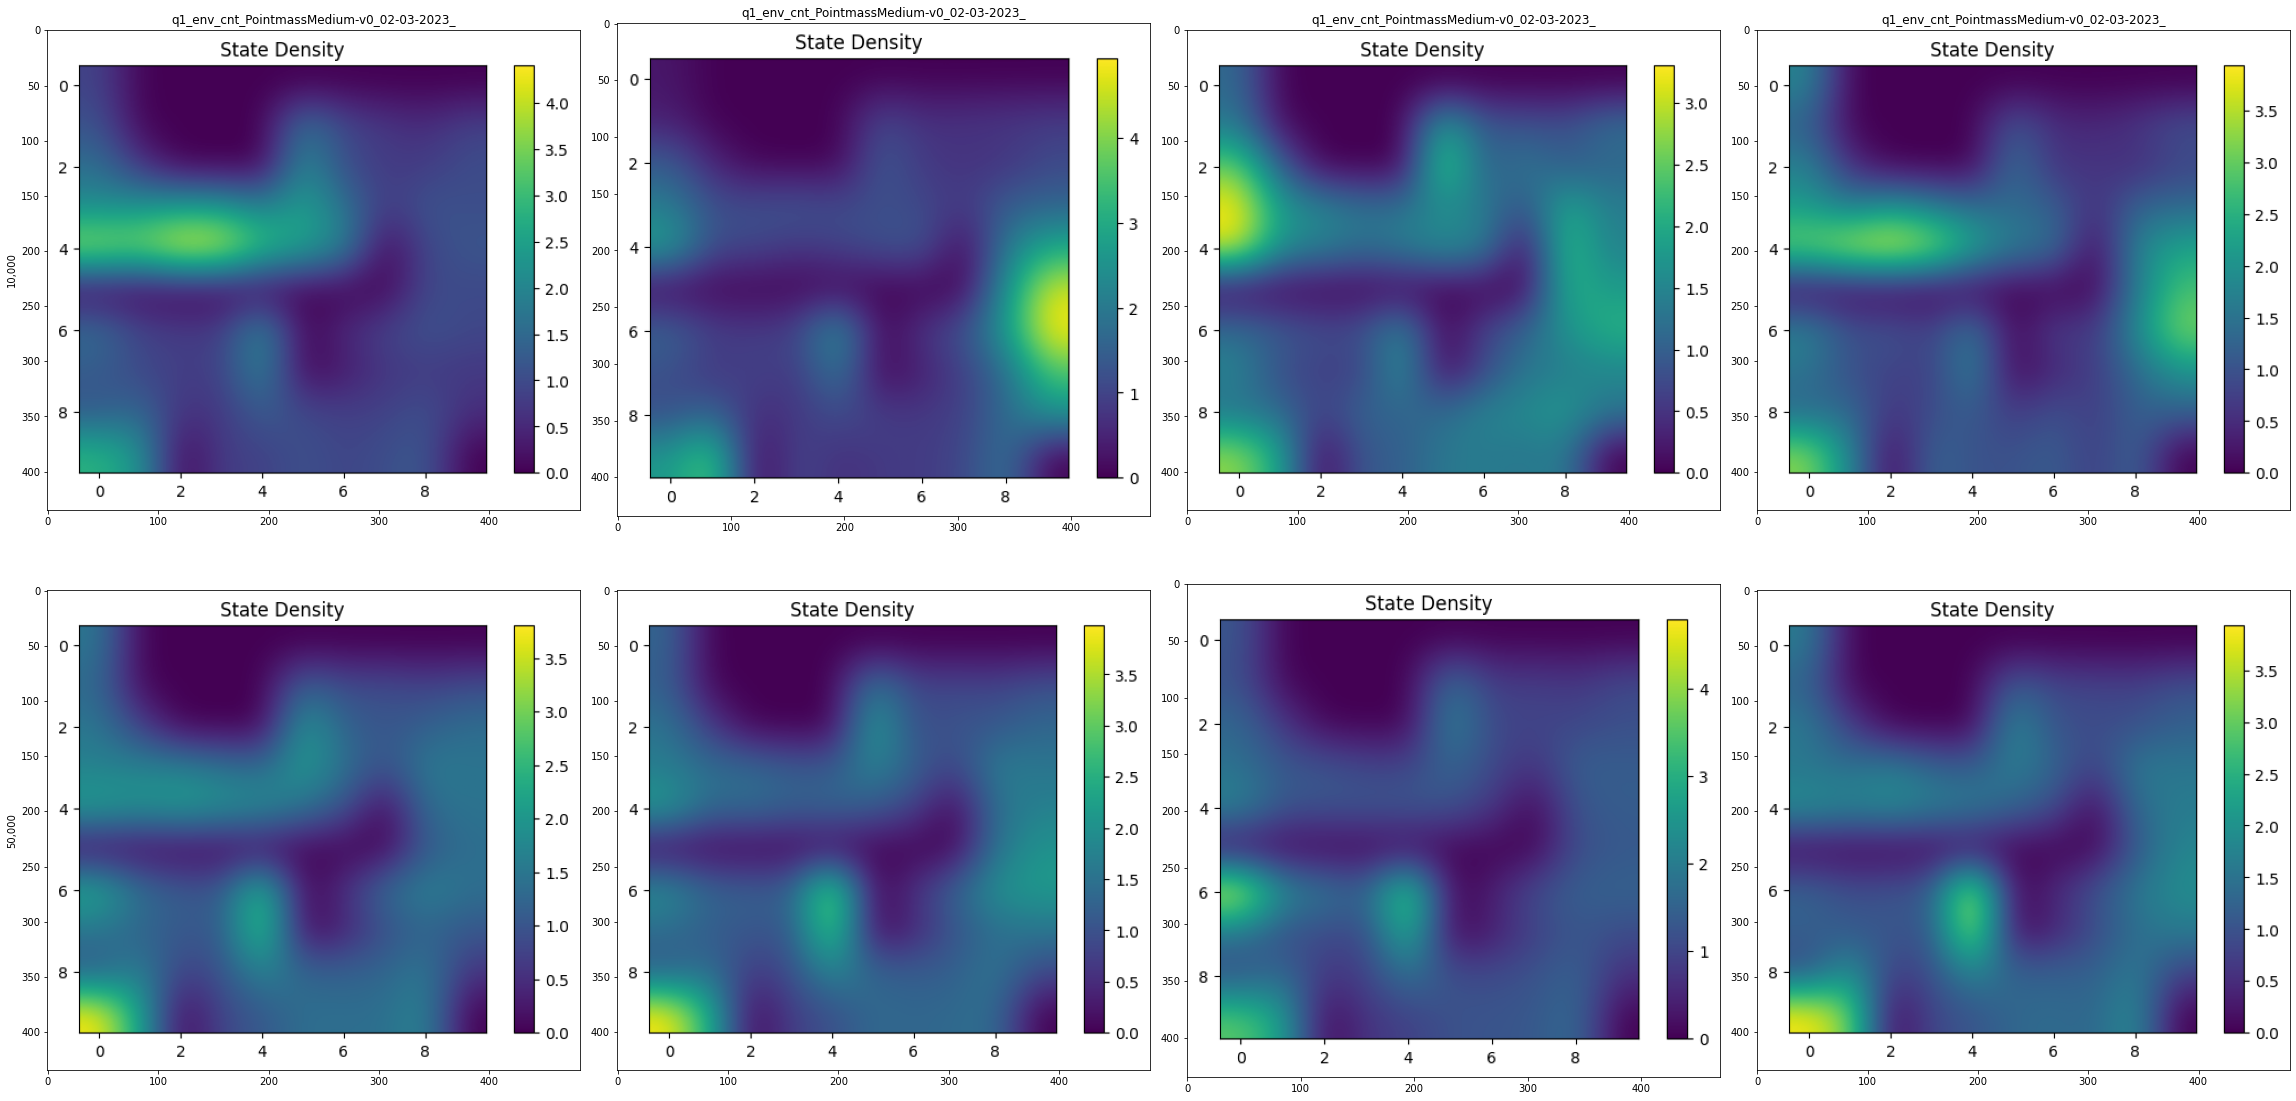
\includegraphics[scale=0.25]{q1/q1-p2-cnt-medium-state-density}

    Count based exploration strategy produces far more uniform state density.
    In terms of training and evaluation performance CNT performs better than RND strategy.
    Performance difference is a result of exploring better.


    \subsubsection*{Hard Environment}

    \hspace*{-0.6in}
    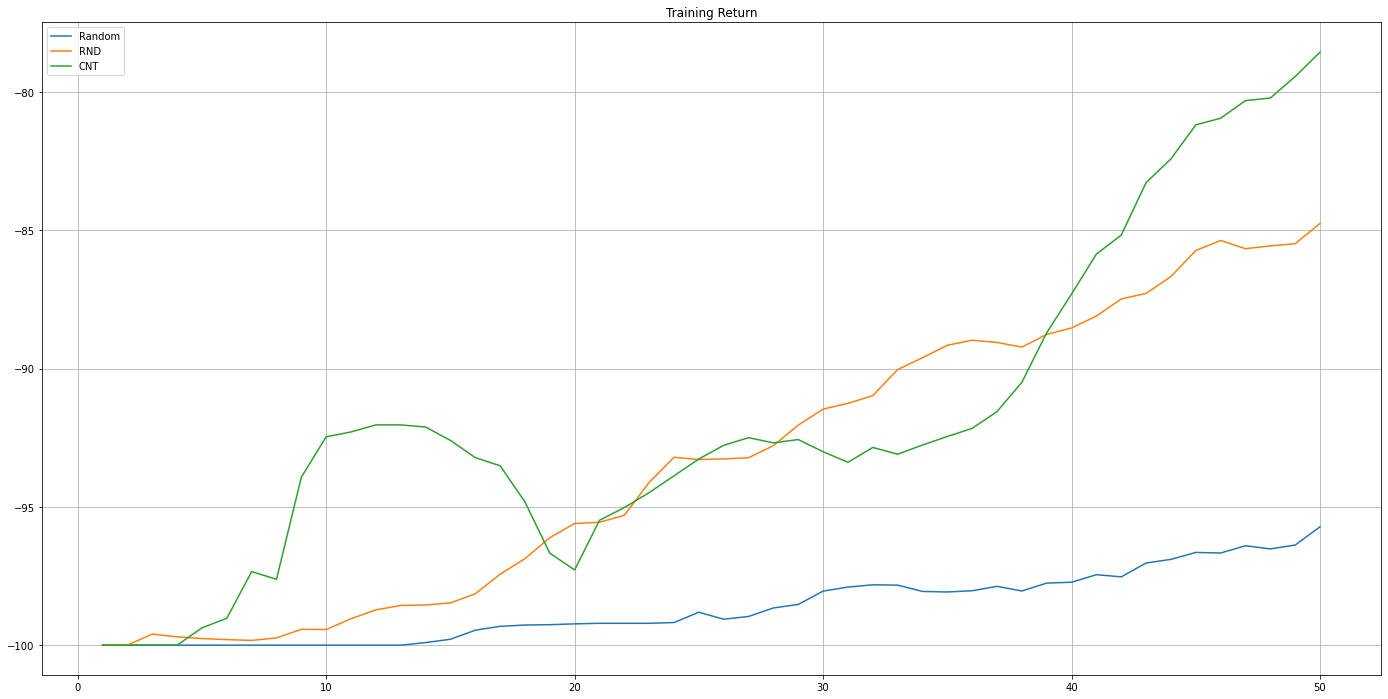
\includegraphics[scale=0.30]{q1/q1-p2-cnt-hard-train}

    \hspace*{-0.6in}
    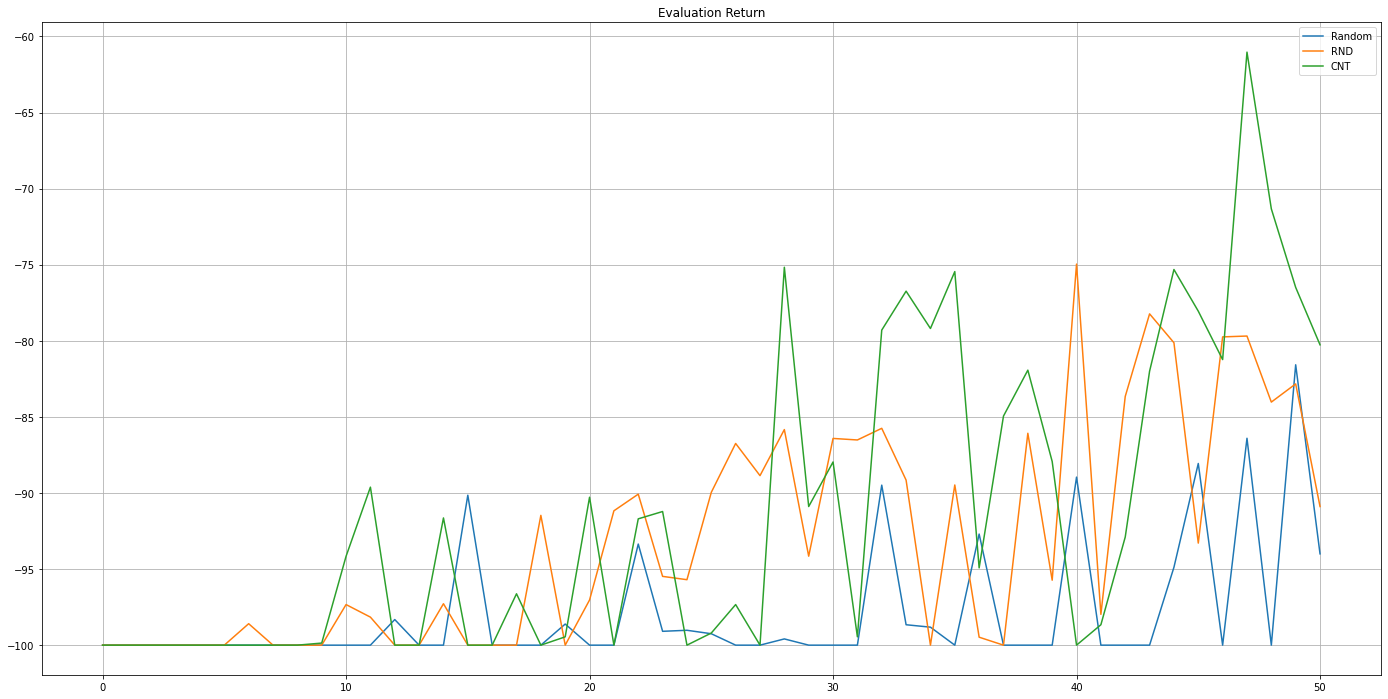
\includegraphics[scale=0.30]{q1/q1-p2-cnt-hard-eval}

    \hspace*{-0.6in}
    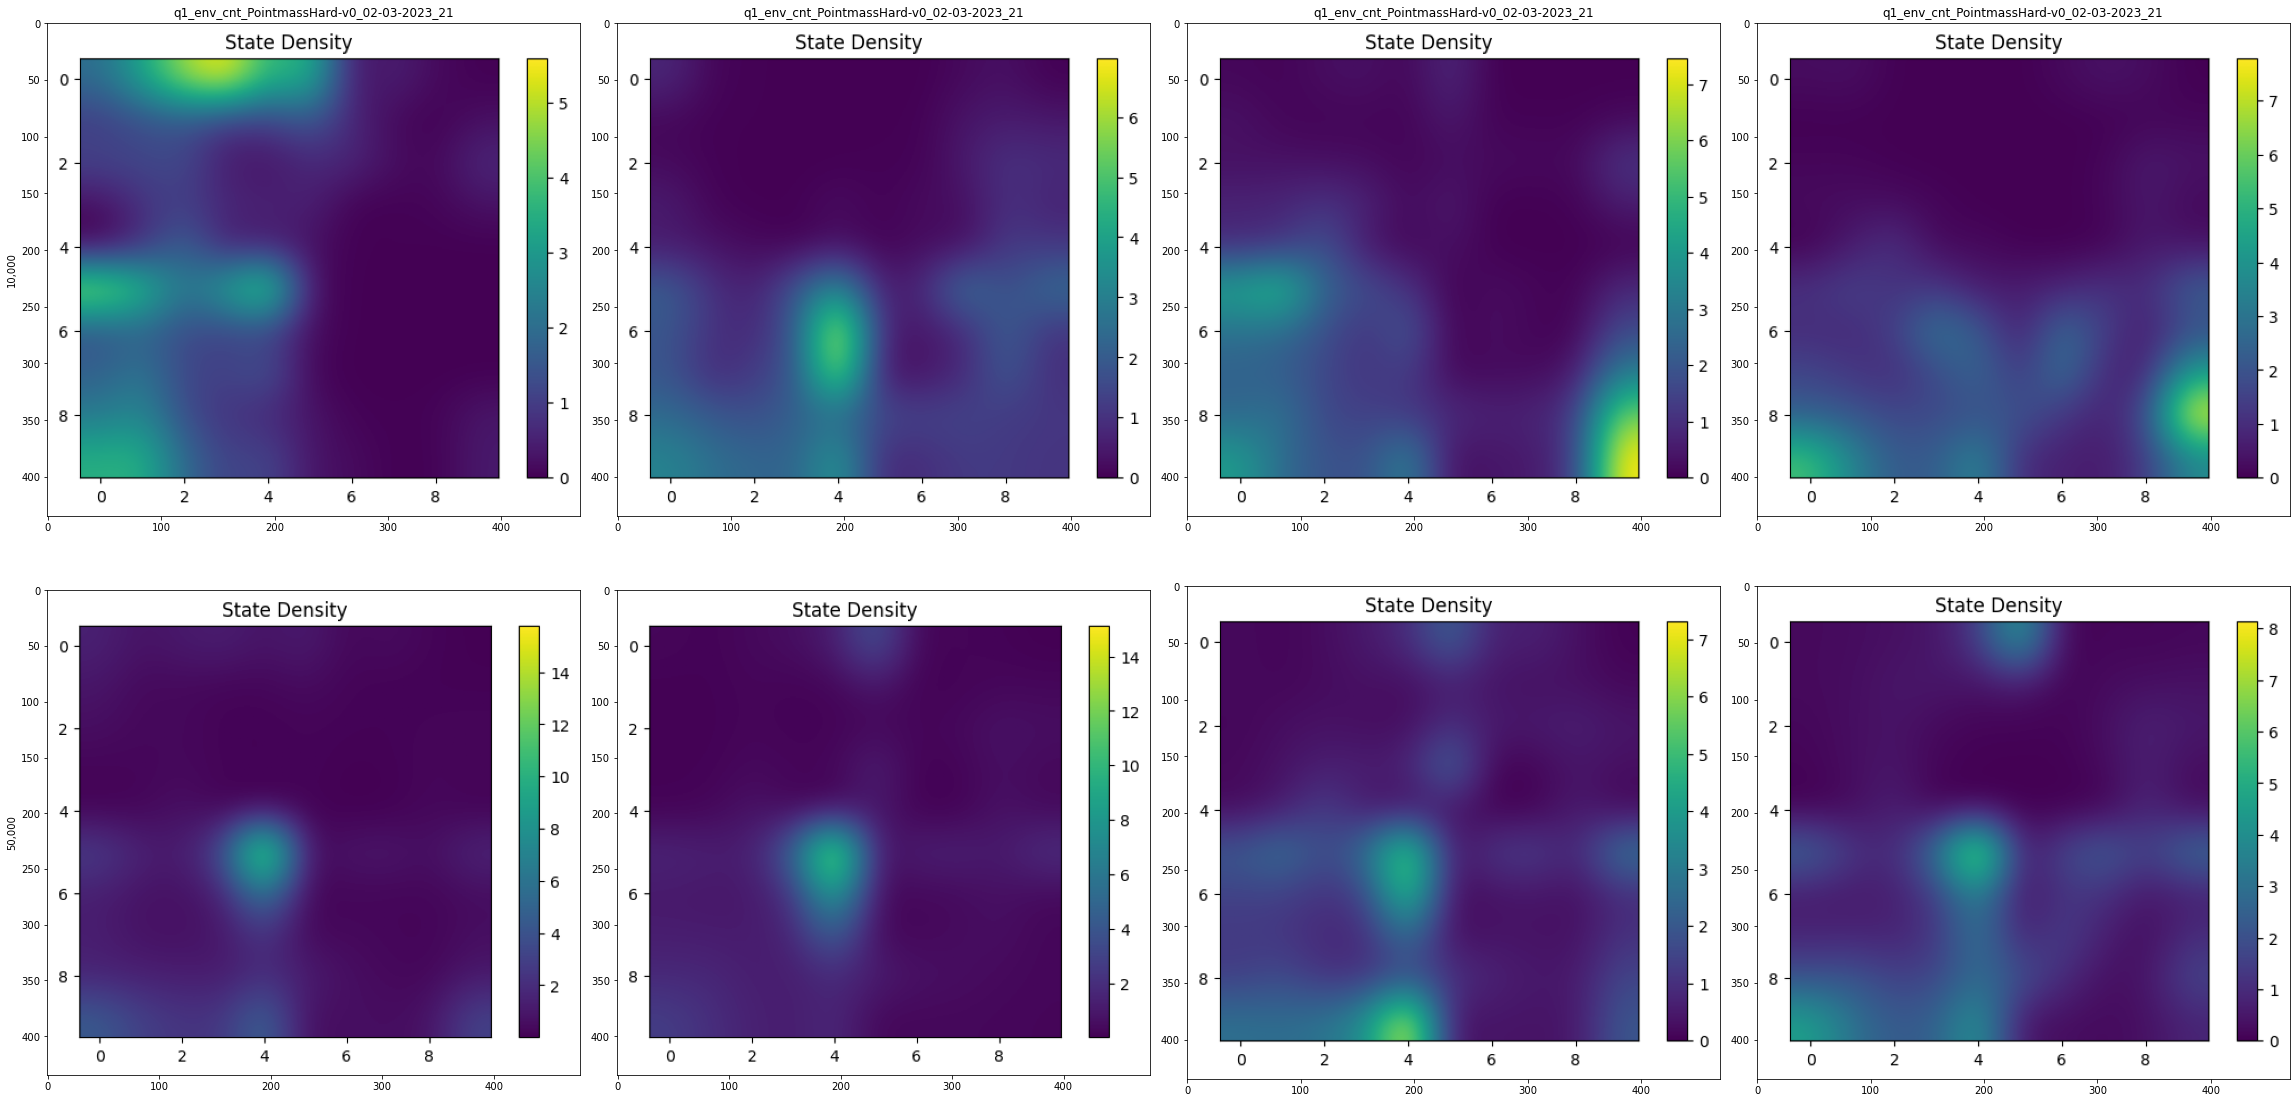
\includegraphics[scale=0.25]{q1/q1-p2-cnt-hard-state-density}

    Count based exploration strategy initially explores better than RND does.
    At the end, count based exploration RND exploration state densities are similar.

    CNT training performance starts better thanks to better exploration.
    CNT training performance degrades after exploitation starts.
    This indicates CNT exploitation critic values are worse that RND exploitation critic values at the beginning of the exploitation.

    \hspace*{-0.6in}
    \includegraphics[scale=0.30]{q1/q1-p2-cnt-hard-intrinsic-rewards}

    Given the similarity of the generated intrinsic rewards (mixed rewards), it is not clear why CNT critic is worse.

    At late stages of the exploitation, CNT exploitation critic values improve.
    Training performance of the CNT catches the RND strategy performance.

    Evaluation performance during exploration also shows that CNT exploitation critic values are worse than RND exploitation critic values.
    CNT evaluation performance follows training performance and catches RND evaluation performance by the end of the training.


\end{document}